\documentclass{article}
\usepackage[utf8]{inputenc}
\usepackage[italian]{babel}
\usepackage{graphicx} % Required for inserting images
\usepackage{float}
\usepackage{datetime}
\usepackage{alltt, fancyvrb, url}
\usepackage{hyperref}
\usepackage{csquotes}
\usepackage{adjustbox}
\usepackage{mdframed}
\usepackage{makeidx}
\usepackage{ifthen} %esecuzioni condizionali
\usepackage{algorithmicx} %algoritmi
\usepackage{algpseudocode} %costrutti pseudocodice
\usepackage{framed, color}
\usepackage{listings} %porzioni di codice 
\usepackage{xfp} %per moltiplicazioni
\usepackage{enumitem}
\usepackage{amsmath,amsfonts,amssymb} % Matematica
\usepackage{xcolor}
\usepackage{tikz} % grafici
\usepackage{parskip}
\usepackage{tcolorbox}
\usepackage[ style=numeric, citestyle=numeric]{biblatex}
\usepackage[italian]{cleveref} % pacchetto per i riferimenti incrociati

\usetikzlibrary{arrows.meta, positioning,fit,trees}

\colorlet{shadecolor}{gray!25}

% Definizione customitemize per Bob e Alice
\newcounter{person}
\newcommand{\person}{%
  \ifnum\value{person}=0 Bob\else Alice\fi%
  \stepcounter{person}%
  \ifnum\value{person}=2 \setcounter{person}{0}\fi%
}
\newlist{customitemize}{itemize}{1}
\setlist[customitemize,1]{label={[\person]},before=\setcounter{person}{0}}

%DECOMMENTA SE VUOI FARE CITAZIONI
%\usepackage[style=verbose-ibid,backend=biber]{biblatex} %per la bibliografia con \cite, \footcite, ecc.
\usepackage[italian]{babel}
\usepackage{xurl} %per linkare url con \url{}
\usepackage{amsmath} % pacchetto per le equazioni matematiche
\usepackage{amsthm}
\theoremstyle{definition}
% Definizione dell'ambiente per le definizioni
\newtheorem{definizione}{Definizione}

\usepackage{amssymb}
%\usepackage{biblatex}
\usepackage[
backend=biber,
style=alphabetic,
sorting=ynt
]{biblatex}

\usepackage[italian]{cleveref} % pacchetto per i riferimenti incrociati

\addbibresource{bibliography.bib}

\title{Secure socket layer \\
        \large
        Corso di Crittografia A.A. 2022/23}
\author{Falconi Eleonora}
\date{\today}

\begin{document}

\maketitle
\clearpage
\tableofcontents
\clearpage



\section{Introduzione}

La crittografia consiste nello studio di metodi matematici associati a vari aspetti della protezione delle informazioni, quali la segretezza, l'integrità dei dati, l'autenticazione delle entità e la verifica dell'origine dei dati.

\textbf{Obbiettivi della crittografia} %LIBRO HANDBOOK PROF CAP 1
I seguenti quattro obbiettivi costituiscono un quadro su cui gli altri saranno derivati: 

1. La \textit{riservatezza } è un servizio utilizzato per mantenere il contenuto delle informazioni al riparo da tutti tranne che da coloro che sono autorizzati a conoscerlo. Il termine "segretezza" è sinonimo di riservatezza e privacy. Esistono diversi approcci per fornire riservatezza, che vanno dalla protezione fisica fino agli algoritmi matematici che rendono i dati incomprensibili.

2. L'\textit{integrità dei dati} affronta l'alterazione non autorizzata dei dati. Per garantire l'integrità dei dati, è necessario avere la capacità di rilevare la manipolazione dei dati da parte di soggetti non autorizzati. La manipolazione dei dati include l'inserimento, la cancellazione e la sostituzione di essi.

3. L'\textit{autenticazione} è un servizio legato all'identificazione. Questa funzione si applica sia alle entità che alle informazioni stesse. Due parti che entrano in comunicazione dovrebbero identificarsi reciprocamente. Le informazioni consegnate su un canale dovrebbero essere autenticate per quanto riguarda l'origine, la data di origine, il contenuto dei dati, l'orario di invio, ecc. Per questi motivi, questo aspetto della crittografia è solitamente suddiviso in due classi principali: \textit{autenticazione delle entità} e \textit{autenticazione dell'origine dei dati}. L'autenticazione dell'origine dei dati fornisce implicitamente l'integrità dei dati ,poiché se un messaggio viene modificato, l'origine è cambiata. Mentre l'autenticazione delle entità significa assicurarsi che ciascuna parte sia effettivamente chi dichiara di essere.

4. La \textit{non-rinnegabilità} è una caratteristica che impedisce a un'entità di negare impegni o azioni precedenti. Quando sorgono dispute a causa di un'entità che nega che siano state prese determinate azioni, è necessario un mezzo per risolvere la situazione. Ad esempio, un'entità può autorizzare l'acquisto di un bene da parte di un'altra entità e successivamente negare di aver concesso tale autorizzazione. È necessaria una procedura che coinvolga una terza parte di fiducia per risolvere la disputa.

\begin{figure}[H]
    \centering
    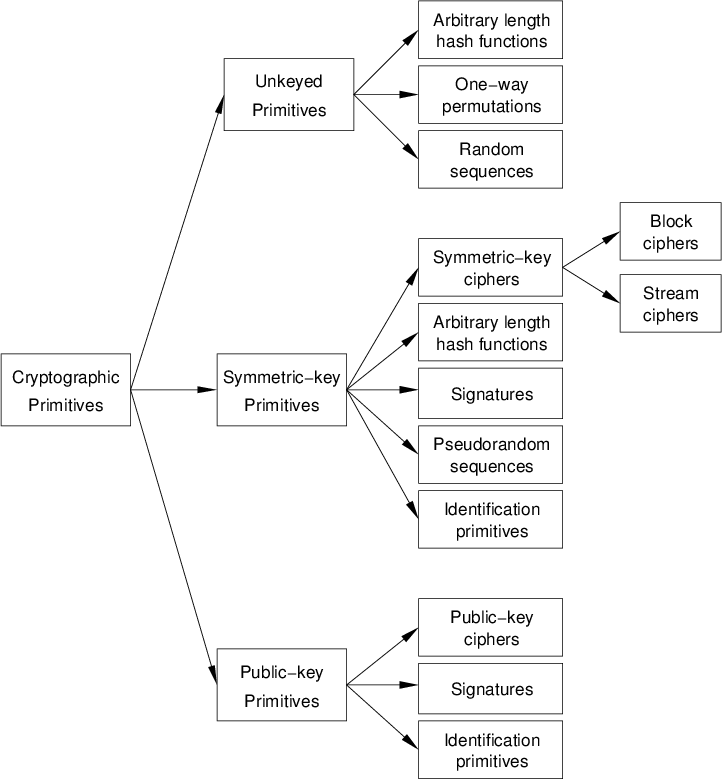
\includegraphics[height=0.5\textheight]{img/taxonomy.png}
    \caption{Tassonomia del primitivi crittografici.}
    \label{fig:itm}
\end{figure}
% La Figura 1. fornisce un elenco schematico delle primitive prese in considerazione e delle loro relazioni. Molte di queste saranno brevemente presentate in questo capitolo, mentre una discussione dettagliata verrà lasciata ai capitoli successivi. Queste primitive dovrebbero essere valutate in base a vari criteri come:

\subsection{Storia}
Il protocollo TCP offre un canale di comunicazione affidabile tra due nodi, in grado di rilevare la perdita o la corruzione dei pacchetti, ma non affronta il problema dell'autenticazione e può essere vulnerabile agli attacchi basati sugli indirizzi.

Nel caso di SSL (Secure Socket Layer), stiamo parlando di un protocollo aperto e non proprietario, sviluppato da Netscape Communication Corporation con l'obiettivo principale di proteggere le comunicazioni sul World Wide Web\footnote{Il World Wide Web("WWW") è un sistema di documenti interconnessi tramite collegamenti ipertestuali, accessibili via internet. I documenti sono scritti in HTML e visualizzati attraverso browser web, utilizzando il protocollo HTTP.}. Nel corso del tempo, sono state presentate diverse iterazioni di questo protocollo:

\begin{itemize}[label={\textbullet}]
  \item 1994: Versione 1 che presentava diversi problemi e mai pubblicata;
  \item 1994: Versione 2 implementata in Netscape Navigator 1;
  \item 1996: Versione 3 implementata in Netscape Navigator 3;
  \item 1999: TLS (Transport Layer Security), evoluzione di SSL proposta dal IETF, che formalizza il protocollo. Nel tempo è stata sottoposta a diverse migliorie, fino alla RFC 3268 che supporta tutte le più moderne tecnologie per la crittografia simmetrica (AES, IDEA, DES e 3DES).
\end{itemize}

\subsection{Terminologia e concetti di base} %da mettere a posto CAP 1 LIBRO PROF HANDBOOK
Questo capitolo introduce alcuni concetti chiave fondamentali per la comprensione dei sistemi crittografici e più nello specifico di SSL.
\subsubsection{Domini e codomini}
Nel mondo della crittografia e della sicurezza delle informazioni, è essenziale disporre di un linguaggio, concetti chiari e ben definiti per comprendere e comunicare in modo efficace. In particolare, verranno esposti tre elementi chiave:

\begin{itemize}[label={\textbullet}]
\item[-] $\mathcal{A}$ rappresenta un insieme finito chiamato \textit{alfabeto di definizione}. Ad esempio, $\mathcal{A} = \{0, 1\}$, l'alfabeto binario, è un alfabeto di definizione spesso utilizzato. È importante notare che qualsiasi alfabeto può essere codificato utilizzando l'alfabeto binario. Infatti, poiché ci sono 32 stringhe binarie di lunghezza cinque, a ciascuna lettera dell'alfabeto inglese può essere assegnata una stringa binaria unica di lunghezza cinque.

\item[-]\texttt{$\mathcal{M}$} rappresenta un insieme chiamato \textit{spazio dei messaggi}. \texttt{$\mathcal{M}$} è costituito da stringhe di simboli provenienti da un alfabeto di definizione. Un elemento di \texttt{$\mathcal{M}$} è chiamato \textit{messaggio in chiaro} o semplicemente messaggio. Ad esempio, \texttt{$\mathcal{M}$} può consistere in stringhe binarie, testo in inglese o codice informatico.

\item[-]\texttt{$\mathcal{C}$} rappresenta un insieme chiamato \textit{spazio dei cifrati}. \texttt{$\mathcal{C}$} è costituito da stringhe di simboli provenienti da un alfabeto di definizione, che può differire dall'alfabeto di definizione di \texttt{$\mathcal{M}$}. Un elemento di \texttt{$\mathcal{C}$} è chiamato \textit{testo cifrato}.
\end{itemize}

\subsubsection{Trasformazioni di cifratura e decifratura}
%VERSIONE 1
\begin{itemize}
    \item \( \mathcal{K} \) denota un insieme chiamato \textit{spazio delle chiavi} e un elemento di \( \mathcal{K} \) è chiamato \emph{chiave}.
    \item Ogni elemento \( e \in \mathcal{K} \) determina in modo univoco una corrispondenza biunivoca\footnote{Una funzione biunivoca stabilisce una corrispondenza perfetta tra gli elementi di due insiemi: ogni elemento dell'insieme di partenza (dominio) corrisponde esattamente a un elemento nell'insieme di arrivo (codominio) e ogni elemento nell'insieme di arrivo proviene esattamente da un elemento dell'insieme di partenza.} da \( \mathcal{M} \) a \( \mathcal{C} \), denotata da \( E_e \). \( E_e \) è chiamata \textit{funzione di crittografia} o \textit{trasformazione di crittografia}. Si noti che \( E_e \) deve avere una corrispondenza biunivoca per poter invertire il processo e recuperare un messaggio in chiaro univoco per ogni testo cifrato distinto\footnote{Maggiore generalità si ottiene se \( E_e \) è semplicemente definita come una trasformazione biunivoca da \( \mathcal{M} \) a \( \mathcal{C} \). In altre parole,
\( E_e \) è una biezione da \( \mathcal{M} \) a Im(\( E_e \)) dove Im(\( E_e \)) è un sottoinsieme di \( \mathcal{C} \).}.
    \item Per ogni \( d \in \mathcal{K} \), \( D_d \) denota una corrispondenza biunivoca da \( \mathcal{C} \) a \( \mathcal{M} \) (cioè, \( D_d: \mathcal{C} \rightarrow \mathcal{M} \)). \( D_d \) è chiamata \textit{funzione di decrittografia} o \textit{trasformazione di decrittografia}.
    \item Il processo di applicazione della trasformazione \( E_e \) a un messaggio \( m \in \mathcal{M} \) è solitamente indicato come la \textit{cifratura} di \( m \).
    \item Il processo di applicazione della trasformazione \( D_d \) a un cifrato \( c \) è solitamente indicato come la \textit{decifratura} di \( c \).
    \item Uno schema di cifratura consiste in un insieme \( \{E_e : e \in \mathcal{K}\} \) di trasformazioni di cifratura e un insieme corrispondente \( \{D_d : d \in \mathcal{K}\} \) di trasformazioni di decifrazione con la proprietà che per ogni \( e \in \mathcal{K} \) esiste una chiave univoca \( d \in \mathcal{K} \) tale che \( D_d = E^{-1}_e \); cioè, \( D_d(E_e(m)) = m \) per ogni \( m \in \mathcal{M} \). Uno schema di cifratura è talvolta indicato come \textit{cifrario}.
    \item Le chiavi \( e \) e \( d \) nella definizione precedente sono indicate come una \textit{coppia di chiavi} e talvolta denotate da \( (e, d) \). Però \( e \) e \( d \) potrebbero essere identiche.
    \item Costruire uno schema di cifratura richiede di selezionare uno spazio dei messaggi \( \mathcal{M} \), uno spazio dei cifrati \( \mathcal{C} \), uno spazio delle chiavi \( \mathcal{K} \), un insieme di trasformazioni di cifratura \( \{E_e : e \in \mathcal{K}\} \), e un insieme corrispondente di trasformazioni di decifrazione \( \{D_d : d \in \mathcal{K}\} \).\cite{domini}
\end{itemize}
%VERSIONE 2 VEDI QUALE ELIMINARE
%\textbf{Spazio delle chiavi} (\texttt{$\mathcal{K}$}): Questo è un insieme chiamato spazio delle chiavi. Un elemento in \texttt{$\mathcal{K}$} è chiamato chiave.

%\textbf{Trasformazione di crittografia} (\texttt{$\mathcal{Ee}$}): Ogni elemento $e \in \mathcal{K}$ determina in modo univoco una corrispondenza uno-a-uno tra il messaggio M e il cifrato C, indicata come Ee. Ee è chiamata funzione di crittografia o trasformazione di crittografia. È importante notare che Ee deve essere una corrispondenza uno-a-uno (bijection) affinché il processo possa essere invertito e si possa recuperare un messaggio in chiaro univoco per ogni cifrato distintivo.

%\textbf{Trasformazione di decrittografia} (\texttt{$\mathcal{Dd}$}): Per ogni $d \in \mathcal{K}$, Dd rappresenta una corrispondenza uno-a-uno tra il cifrato C e il messaggio M (cioè, Dd: C → M). Dd è chiamata funzione di decrittografia o trasformazione di decrittografia.

%\textbf{Crittografia di un messaggio} (Ee): Il processo di applicazione della trasformazione Ee a un messaggio $m \in \mathcal{M}$ è comunemente chiamato crittografare m o cifrare m.

%\textbf{Decrittografia di un cifrato} (Dd): Il processo di applicazione della trasformazione Dd a un cifrato c è comunemente chiamato decrittografare c o decifrare c.

%\textbf{Schema di crittografia} : Uno schema di crittografia è composto da un insieme $\{E_e: e \in \mathcal{K}\}$ di trasformazioni di crittografia e un insieme corrispondente $\{D_d: d \in \mathcal{K}\}$ di trasformazioni di decrittografia. Questi insiemi devono soddisfare la proprietà che per ogni $e \in \mathcal{K}$ esiste una chiave $d$ univocamente associata in $\mathcal{K}$ tale che $D_d = E_e^{-1}$, il che significa che $D_d(E_e(m)) = m$ per ogni $m \in M$. Uno schema di crittografia è talvolta chiamato cifra.

%\textbf{Coppia di chiavi} Coppia di chiavi (e, d): Le chiavi e d nella definizione precedente sono chiamate coppia di chiavi e a volte sono indicate come (e, d). È importante notare che e e d potrebbero essere gli stessi.

%\textbf{Costruzione di uno schema di crittografia} : Per costruire uno schema di crittografia, è necessario selezionare uno spazio di messaggi M, uno spazio di cifrati C, uno spazio di chiavi K, un insieme di trasformazioni di crittografia {Ee: $e \in \mathcal{K}$}, e un insieme corrispondente di trasformazioni di decrittografia {Dd: $d \in \mathcal{K}$}.


\subsection{Cifrari simmetrici e asimmetrici}
Verrà riportata di seguito una descrizione dei cifrari di tipo simmetrico e cifrari di tipo asimmetrico.
\subsubsection{Cifrari a chiave segreta o simmetrici}

Consideriamo uno schema di cifratura composto dagli insiemi di trasformazioni di cifratura e decifratura\(\{E_e : e \in \mathcal{K}\}\) e \(\{D_d : d \in \mathcal{K}\}\), rispettivamente, dove \( \mathcal{K} \) è lo \textit{spazio delle chiavi}. Lo schema di cifratura è detto a \textit{chiave simmetrica} se per ogni coppia associata di chiavi di cifratura/decifratura \((e, d)\) è computazionalmente "facile" determinare \(d\) conoscendo solo \(e\), e viceversa.
Poiché nella maggior parte degli schemi di cifratura simmetrica pratici si ha 
\begin{equation*}
e = d
\end{equation*}

il termine chiave simmetrica diventa appropriato. Le tecniche di crittografia a chiave simmetrica più conosciute sono i cifrari a blocchi. Un \textit{cifrario a blocchi} è uno schema di cifratura che suddivide i messaggi in chiaro da trasmettere in stringhe (chiamate blocchi) di lunghezza fissa \( t \) su un alfabeto \( \mathcal{A} \) che effettua la cifratura di un blocco alla volta. 

Due importanti classi di cifrari a blocchi sono i \textit{cifrari a sostituzione} e i \textit{cifrari a trasposizione}.

\paragraph{Cifrari di sostituzione semplici}  Sia $\mathcal{A}$ un alfabeto di \( q \) simboli e $\mathcal{M}$ l'insieme di tutte le stringhe di lunghezza \( t \) su $\mathcal{A}$. Sia $\mathcal{K}$ l'insieme di tutte le permutazioni sull'insieme $\mathcal{A}$. Definiamo per ogni \( e \in \mathcal{K} \) una trasformazione di cifratura \( E_e \) come:
\[
E_e(m)=(e(m_1)e(m_2) \ldots e(m_t)) = (c_1c_2 \ldots c_t) = c,
\]
dove \( m = (m_1m_2 \ldots m_t) \in \mathcal{M} \). In altre parole, per ogni simbolo di una \( t \)-tupla, sostituirlo con un altro simbolo di $\mathcal{A}$ secondo una permutazione fissa \( e \). Per decifrare \( c = (c_1c_2 \ldots c_t) \) calcolare la permutazione inversa \( d = e^{-1} \) e
\[
D_d(c)=(d(c_1)d(c_2) \ldots d(c_t)) = (m_1m_2 \ldots m_t) = m.
\]
\( E_e \) è chiamato un cifrario di sostituzione semplice o un cifrario di sostituzione monoalfabetico.

Il numero di cifrari di sostituzione distinti è $q!$ ed è indipendente dalla dimensione del blocco nel cifrario. Il cifrario di sostituzione semplice di lunghezza di blocco cinque ne è un esempio. I cifrari di sostituzione semplice su dimensioni di blocco piccole offrono una sicurezza inadeguata anche quando lo spazio chiave è estremamente ampio. Se l'alfabeto è quello inglese, allora la dimensione dello spazio chiave è $26! \approx 4 \times 10^{26}$, tuttavia la chiave utilizzata può essere determinata piuttosto facilmente esaminando una modesta quantità di testo cifrato. Questo deriva dalla semplice osservazione che la distribuzione delle frequenze delle lettere viene conservata nel testo cifrato. Ad esempio, la lettera E si verifica più frequentemente delle altre lettere in un testo inglese ordinario. Di conseguenza, la lettera che si verifica con maggiore frequenza in una sequenza di blocchi di testo cifrato corrisponde molto probabilmente alla lettera E nel testo in chiaro. Osservando una modesta quantità di blocchi di testo cifrato, un crittografo può determinare la chiave.


%\paragraph{Cifrari di sostituzione omofonica} CAP 1 HANDBOOK

%In un cifrario di sostituzione omofonica, ogni simbolo \( a \) preso da un insieme $\mathcal{A}$ è associato a un insieme di stringhe \( H(a) \) di lunghezza \( t \). L'importante è che questi insiemi di stringhe siano tutti distinti, ovvero non condividano stringhe tra di loro per differenti simboli \( a \). Quando si cifra un messaggio, ogni simbolo \( a \) viene sostituito da una delle stringhe in \( H(a) \), scelta in modo casuale. Al contrario, quando si decifra, si cerca il simbolo \( a \) corrispondente identificando a quale insieme \( H(a) \) appartiene la stringa cifrata \( c \). La chiave che determina come avviene la cifratura e decifratura è data dagli insiemi specifici \( H(a) \).

%\paragraph{Cifrari di sostituzione polialfabetica}
%Un cifrario di sostituzione polialfabetica è un cifrario a blocchi con lunghezza del blocco \( t \) su un alfabeto \( A \) avente le seguenti proprietà:
%\begin{enumerate}
    %\item lo spazio delle chiavi $\mathcal{K}$ consiste in tutti gli insiemi ordinati di \( t \) permutazioni \((p_1, p_2,... ,p_t)\), dove ogni permutazione \( p_i \) è definita sull'insieme $\mathcal{A}$;
   % \item la cifratura del messaggio \( m = (m_1 m_2 \ldots m_t) \) sotto la chiave \( e = (p_1, p_2,... ,p_t) \) è data da \( E_e(m) = (p_1(m_1) p_2(m_2) \ldots p_t(m_t)) \); e
   % \item la chiave di decrittografia associata a \( e = (p_1, p_2,... ,p_t) \) è \( d = (p_1^{-1}, p_2^{-1},... ,p_t^{-1}) \).
%\end{enumerate}

\paragraph{Cifrari di trasposizione}
Un'altra classe di cifrari a chiave simmetrica è il cifrario di trasposizione semplice, il quale permuta semplicemente i simboli all'interno di un blocco.

Consideriamo uno schema di cifratura a blocchi a chiave simmetrica con lunghezza del blocco \( t \). Sia \( \mathcal{K} \) l'insieme di tutte le permutazioni sull'insieme \(\{1, 2, \ldots, t\}\). Per ogni \( e \in \mathcal{K} \), definiamo la funzione di cifratura 
\begin{equation}
    E_e(m) = (m_{e(1)} m_{e(2)} \ldots m_{e(t)})
\end{equation}
dove \( m = (m_1 m_2 \ldots m_t) \in \mathcal{M} \), lo spazio dei messaggi. L'insieme di tutte queste trasformazioni è chiamato cifrario di trasposizione semplice. La chiave di decrittografia corrispondente a \( e \) è la permutazione inversa \( d = e^{-1} \). Per decifrare \( c = (c_1 c_2 \ldots c_t) \in \mathcal{C} \), si calcola \( D_d(c) = (c_{d(1)} c_{d(2)} \ldots c_{d(t)}) \).

Un cifrario di trasposizione semplice conserva il numero di simboli di un dato tipo all'interno di un blocco, rendendolo quindi suscettibile ad analisi crittografica.


\subsubsection{Cifrari a chiave pubblica}
Siano \( \{ E_e : e \in   \mathcal{K} \} \) un insieme di trasformazioni di cifratura e \( \{ D_d : d \in \mathcal{K} \} \) l'insieme delle trasformazioni di decifrazione corrispondenti, dove  \( \mathcal{K} \) è lo spazio delle chiavi. Considera qualsiasi coppia di trasformazioni di cifratura/decifrazione associate \( (E_e, D_d) \) e supponiamo che ogni coppia abbia la proprietà tale che, conoscendo \( E_e \), sia computazionalmente impossibile, dato un cifrato casuale \( c \in C \), trovare il messaggio \( m \in  \mathcal{M} \) tale che \( E_e(m) = c \). Questa proprietà implica che dato \( e \) è impossibile determinare la chiave di decifrazione corrispondente \( d \). \( E_e \) viene qui visto come una funzione \textit{trapdoor one way}\footnote{Una funzione trapdoor(con trappola) unidirezionale  è una funzione unidirezionale \( f : X \rightarrow Y \) con la proprietà aggiuntiva che, date alcune informazioni aggiuntive (chiamate informazioni della trappola), diventa fattibile trovare, per un dato \( y \in \text{Im}(f) \), un \( x \in X \) tale che \( f(x) = y \).
} con \( d \) come informazione \textit{trapdoor} necessaria per calcolare la funzione inversa e quindi consentire la decifrazione. Questo è diverso dai cifrari a chiave simmetrica dove \( e \) e \( d \) sono essenzialmente gli stessi.

Consideriamo ad esempio la comunicazione tra due parti, Alice e Bob. 

\begin{customitemize}
    \item : Sceglie la coppia di chiavi $(e, d)$. Invia la chiave di cifratura $e$ (chiamata chiave pubblica) ad Alice attraverso qualsiasi canale, ma tiene segreta e sicura la chiave di decifrazione $d$ (chiamata chiave privata).
    
    \item : Riceve la chiave pubblica $e$. Successivamente, può inviare un messaggio $m$ cifrandolo con la chiave pubblica $e$ per ottenere $c = E_e(m)$.
    
    \item : Decifra il testo cifrato $c$ applicando la trasformazione inversa $D_d$ univocamente determinata da $d$. Anche se la chiave di cifratura è stata trasmessa attraverso un canale non sicuro, dal momento che non è necessario mantenerla segreta, può essere resa pubblica. Così, chiunque può inviargli messaggi cifrati che solo lui può decifrare.
\end{customitemize}



Se ad esempio un'entità $A1$ cifra un messaggio $m1$ ottenendo $c1$ e poi distrugge $m1$, nemmeno $A1$ può recuperare $m1$ da $c1$. Questo può essere paragonato a una scatola metallica con il coperchio bloccato da una combinazione conosciuta solamente da Bob. Se il lucchetto viene lasciato aperto e reso pubblico, chiunque può mettere un messaggio all'interno e bloccare il coperchio. Ma solo Bob potrà recuperare il messaggio, poichè anche le altre entità che hanno inserito il messaggio nella scatola non potranno recuperarlo.

La crittografia a chiave pubblica, come descritta qui, presuppone che la conoscenza della chiave pubblica \( e \) non permetta il calcolo della chiave privata \( d \). In altre parole, ciò presuppone l'esistenza di funzioni monodirezionali a trappola "trapdoor one way".

%GUARDA SE DA TOGLIERE A ME SEMBRA RIPETIZIONE
\paragraph{Definizione} Consideriamo uno schema di cifratura composto dagli insiemi di trasformazioni di cifratura e decifrazione \( \{ E_e : e \in K \} \) e \( \{ D_d : d \in K \} \), rispettivamente. Si dice che il metodo di cifratura sia uno schema di cifratura a chiave pubblica se, per ogni coppia associata di cifratura/decifrazione \( (e, d) \), una chiave \( e \) (la chiave pubblica) viene resa pubblicamente disponibile, mentre l'altra \( d \) (la chiave privata) viene mantenuta segreta. Perché lo schema sia sicuro, deve essere computazionalmente irrealizzabile calcolare \( d \) da \( e \).

\paragraph{La necessità dell'autenticazione nei sistemi a chiave pubblica.}
Sembra che la crittografia a chiave pubblica sia un sistema ideale, che non richieda un canale sicuro per trasmettere la chiave di cifratura. Questo implicherebbe che due entità potrebbero comunicare su un canale non protetto senza mai essersi incontrate per scambiarsi le chiavi. Sfortunatamente questo non è il caso, poichè un avversario attivo potrebbe sconfiggere il sistema decifrando messaggi destinati a una seconda entità senza rompere il sistema di cifratura. Questo è un tipo di impersonazione ed è un esempio di fallimento del protocollo. In questo scenario l'avversario impersona l'entità B inviando all'entità A una chiave pubblica \( e_0 \) che A assume erroneamente sia la chiave pubblica di B. L'avversario intercetta messaggi cifrati da A a B, decifra con la sua propria chiave privata \( d_0 \), ricalcola la cifratura del messaggio con la chiave pubblica  \( e \) di B, e lo invia a B. Questo evidenzia la necessità di autenticare le chiavi pubbliche per ottenere l'autenticazione dell'origine dei dati delle chiavi pubbliche stesse. A deve essere convinta di cifrare con la legittima chiave pubblica di B.

\begin{figure}[H]
    \centering
    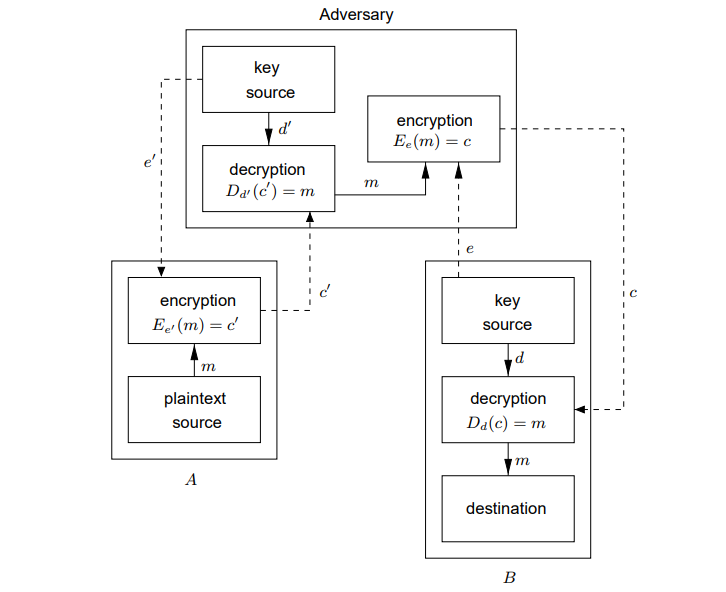
\includegraphics[width=\textwidth]{img/kkk.png}
    \caption{Attacco in una comunicazione tra due parti}
    \label{fig:itm}
\end{figure}

\subsection{Crittografia a chiave simmetrica vs. crittografia a chiave pubblica}

La crittografia a chiave simmetrica e a chiave pubblica ha vari vantaggi e svantaggi, alcuni dei quali sono comuni ad entrambi. Questa sezione evidenzia alcuni di questi e riassume le caratteristiche evidenziate nelle sezioni precedenti.

\paragraph{Vantaggi della crittografia a chiave simmetrica}
\begin{enumerate}
    \item I cifrari con chiave simmetrica sono progettati per garantire un'elevata velocità di trasmissione dei dati. Mentre alcune versioni basate su hardware possono cifrare dati a velocità di centinaia di megabyte al secondo, le imlementazioni software possono raggiungere velocità di throughput nell'ordine dei megabyte al secondo.
    
    \item La dimensione delle chiavi nei cifrari simmetrici è solitamente di lunghezza contenuta.
    
    \item Questi cifrari possono funzionare come elementi di base per creare diverse soluzioni crittografiche, come generatori di numeri pseudocasuali, funzioni di hash e schemi di firma digitale efficienti.
    
    \item Utilizzando combinazioni di cifrari a chiave simmetrica, è possibile ottenere soluzioni di cifratura ancora più robuste. Ciò significa che trasformazioni semplici, anche se deboli da sole, possono essere combinate per ottenere cifrari complessivamente più forti.
    
    \item La cifratura con chiave simmetrica ha radici storiche profonde. Tuttavia, è importante notare che gran parte delle innovazioni in questo settore sono avvenute dopo l'avvento dei computer digitali, specialmente dopo la creazione dello Standard di Cifratura dei Dati negli anni '70.
\end{enumerate}

\paragraph{Svantaggi della crittografia a chiave simmetrica}\label{TTP}
\begin{enumerate}
    \item In una comunicazione tra due entità, la chiave deve rimanere segreta ad entrambe le estremità.
    \item In una grande rete ci sono molte coppie di chiavi da gestire, di conseguenza una gestione efficace delle chiavi richiede l'uso di un TTP(\textit{"Trusted Third Party"}, ovvero \textit{"terza parte fidata"}) incondizionatamente fidato\footnote{Ente o entità che viene considerata completamente affidabile senza riserve o condizioni.}.
    \item In una comunicazione tra le entità A e B una buona pratica crittografica impone di cambiare frequentemente la chiave, meglio se ogni sessione di comunicazione.
    \item I meccanismi di firma digitale derivanti dalla cifratura a chiave simmetrica tipicamente richiedono chiavi più grandi per la funzione di verifica pubblica o l'uso di un TTP.
\end{enumerate}

\paragraph{Vantaggi della crittografia a chiave pubblica}
\begin{enumerate}
    \item Solo la chiave privata deve rimanere riservata. Tuttavia, l'autenticità delle chiavi pubbliche deve essere garantita.
    
    \item Per gestire le chiavi in una rete è sufficiente un TTP funzionalmente fidato (si veda paragrafo precedente \ref{TTP}), a differenza di un TTP incondizionatamente fidato. A seconda della modalità di utilizzo, potrebbe essere necessario ricorrere al TTP solo in modalità "offline" invece che in tempo reale.
    
    \item A seconda della modalità di utilizzo, una coppia di chiavi privata o pubblica che sia, può rimanere invariata per lunghi periodi, ad esempio per molte sessioni o addirittura per diversi anni.
    
    \item Numerosi schemi a chiave pubblica offrono meccanismi di firma digitale relativamente efficienti. La chiave utilizzata per descrivere la funzione di verifica pubblica è in genere molto più piccola rispetto all'equivalente chiave simmetrica.
    
    \item In una vasta rete, il numero totale di chiavi necessarie potrebbe essere notevolmente inferiore rispetto allo scenario con chiavi simmetriche.
\end{enumerate}

\paragraph{Svantaggi della crittografia a chiave pubblica}
\begin{enumerate}
    \item Le velocità di throughput per i metodi di cifratura a chiave pubblica più popolari sono di diversi ordini di grandezza più lenti rispetto ai migliori schemi a chiave simmetrica conosciuti.
    \item Le dimensioni delle chiavi sono tipicamente molto più grandi di quelle richieste per la cifratura a chiave simmetrica.
    \item Nessuno schema a chiave pubblica è stato dimostrato essere sicuro. I migliori schemi di cifratura a chiave pubblica trovati fino ad oggi basano la loro sicurezza sulla presunta difficoltà di un piccolo insieme di problemi di teoria dei numeri.
    \item La crittografia a chiave pubblica non ha una storia così estesa come la cifratura a chiave simmetrica, essendo stata scoperta solo a metà degli anni '70.
\end{enumerate}

\paragraph{Conclusione}
La cifratura con chiave simmetrica e con chiave pubblica hanno una serie di vantaggi complementari, poiché gli attuali sistemi crittografici sfruttano i punti di forza di ciascuno di essi. Di seguito viene fornito un esempio per una maggior comprensione.

Le tecniche di cifratura con chiave pubblica possono essere utilizzate per stabilire una chiave per un sistema a chiave simmetrica utilizzato dalle entità comunicanti \( A \) e \( B \). In questo scenario \( A \) e \( B \) possono trarre vantaggio dalla natura a lungo termine delle chiavi pubbliche/private del sistema a chiave pubblica e dalle efficienze prestazionali del sistema a chiave simmetrica. Poiché la cifratura dei dati è spesso la parte più dispendiosa in termini di tempo del processo di cifratura, lo schema a chiave pubblica per la stabilizzazione della chiave rappresenta una piccola frazione del processo di cifratura tra \( A \) e \( B \).

Ad oggi, la performance computazionale della cifratura con chiave pubblica è inferiore a quella della cifratura con chiave simmetrica. Tuttavia, non esiste alcuna prova che ciò debba necessariamente essere il caso. Ricapitolando:
\begin{enumerate}
    \item La crittografia a chiave pubblica facilita le firme efficienti (in particolare la non ripudiabilità\footnote{La ripudiabilità in crittografia si riferisce alla capacità di negare autenticamente un'azione o un evento. In termini di comunicazione, ciò significa che un mittente può negare di aver inviato un messaggio, e il destinatario non ha alcun modo di dimostrare il contrario, nonostante abbia ricevuto e decifrato correttamente il messaggio.}) e la gestione delle chiavi.
    \item La crittografia a chiave simmetrica è efficiente per la cifratura e per alcune applicazioni di integrità dei dati.
\end{enumerate}

\subsection{Algebra modulare}
Gli interi modulo \( n \), denotati \( \mathbb{Z}_n \), sono l'insieme delle (classi di equivalenza di) interi \{0, 1, 2, \ldots, n - 1\}. L'addizione, la sottrazione e la moltiplicazione in \( \mathbb{Z}_n \) sono eseguite modulo \( n \). Quindi:
\begin{equation*}
    \mathbb{Z}_n = \{0,1,\dots ,n-1\}
\end{equation*}

Sia
\begin{equation*}
a \in \mathbb{Z}_n
\end{equation*}

L'inverso moltiplicativo di \( a \) modulo \( n \) è un intero \( x \in \mathbb{Z}_n \) tale che \( ax \equiv 1 \pmod{n} \). Se tale \( x \) esiste, allora è unico, e \( a \) si dice invertibile, o una unità; l'inverso di \( a \) è denotato da \( a^{-1} \).



\paragraph{Definizione}
Il \emph{modulo}, denotato come \emph{mod}, è un concetto fondamentale in matematica che trova applicazioni in diversi campi, come la teoria dei numeri, l'algebra e, in particolare, la crittografia. Esso è un operatore matematico che determina il resto della divisione euclidea tra due numeri interi.

Dati due interi $a$ e $n$ con $n > 0$, l'operazione $a \bmod n$ restituisce il resto $r$ della divisione di $a$ per $n$. Formalmente, si può esprimere come:
\begin{equation*}
    a \bmod n = r \quad \text{dove} \quad 0 \leq r < n
\end{equation*}

In questo contesto, $a$ è chiamato \emph{dividendo}, $n$ è il \emph{divisore}, e $r$ è il \emph{resto}. Il numero $r$ è l'unico numero non negativo minore di $n$ che soddisfa la seguente relazione di equivalenza:
\begin{equation*}
    a - r \equiv 0 \bmod n
\end{equation*}

In altre parole, $a$ e $r$ sono congruenti modulo $n$ se la loro differenza è un multiplo di $n$. Questo implica che esiste un intero $k$ tale che:
\begin{equation*}
    a - r = k \cdot n
\end{equation*}

Il modulo è particolarmente utile quando si lavora con interi in un intervallo limitato, permettendo di operare in modo ciclico all'interno di questo intervallo. Questa proprietà è essenziale in crittografia, dove l'aritmetica modulare è spesso utilizzata per creare algoritmi di cifratura robusti e efficienti.

\paragraph{Esempio}Un esempio pratico dell'operazione di modulo è l'orologio a 12 ore, dove le ore sono rappresentate come numeri modulo 12. In questo sistema, 13 ore sono equivalenti a 1 ora, poiché $13 \bmod 12 = 1$.

In conclusione il modulo è uno strumento matematico versatile che permette di manipolare numeri interi all'interno di un insieme finito e ciclico, fornendo la base per molte applicazioni matematiche e informatiche.


\subsubsection{Congruenza Modulare}
La \emph{congruenza modulare} è un concetto centrale nella teoria dei numeri e gioca un ruolo fondamentale in vari campi della matematica, dell'informatica e, in particolare, della crittografia. Essa fornisce un modo per comparare numeri interi all'interno di un sistema numerico modulare.

Due numeri interi $a$ e $b$ sono detti \emph{congruenti modulo} $n$, con $n$ un numero naturale positivo, se la loro differenza è un multiplo di $n$. In termini matematici, si scrive:
\begin{equation*}
    a \equiv b \bmod n \Leftrightarrow n \mid (a - b)
\end{equation*}
dove il simbolo $n \mid (a - b)$ denota che $n$ divide $(a - b)$, cioè che la differenza $(a - b)$ è un multiplo intero di $n$.

In altre parole, $a$ e $b$ sono congruenti modulo $n$ se esiste un intero $k$ tale che:
\begin{equation*}
    a = b + kn
\end{equation*}

La congruenza modulare possiede diverse proprietà algebriche interessanti, analoghe a quelle delle equazioni. Per esempio, se $a \equiv b \bmod n$ e $c \equiv d \bmod n$, allora vale che:
\begin{align}
    a + c &\equiv b + d \bmod n \\
    a - c &\equiv b - d \bmod n \\
    ac &\equiv bd \bmod n
\end{align}

Queste proprietà rendono la congruenza modulare uno strumento potente per la manipolazione e l'analisi di numeri interi, specialmente in contesti dove è necessario lavorare con classi di equivalenza di numeri, piuttosto che con i numeri stessi.

Un'applicazione significativa della congruenza modulare si trova nella crittografia a chiave pubblica, dove è utilizzata per creare funzioni unidirezionali, che sono facili da computare in un verso, ma computazionalmente difficili nel verso opposto, a meno di possedere informazioni aggiuntive.

In conclusione, la congruenza modulare è un concetto matematico ricco e versatile che permette di classificare gli interi in base alle loro proprietà residue, offrendo un framework robusto per l'analisi e la manipolazione di numeri interi in una varietà di applicazioni pratiche e teoriche.

\subsubsection{Operazioni Modulari}
Le operazioni modulari, fondamentali in algebra e crittografia, permettono di eseguire operazioni aritmetiche standard in un contesto modulare. Esse includono l'addizione, la sottrazione, la moltiplicazione e, in certi casi specifici, la divisione.

\paragraph{Addizione Modulare}
L'addizione modulare è un'operazione binaria che combina due interi in modulo $n$.
È definita come:
\begin{equation*}
    (a + b) \bmod n = (a \bmod n + b \bmod n) \bmod n
\end{equation*}
Questa operazione è commutativa e associativa, il che significa che l'ordine degli addendi non influisce sul risultato, e che il modo in cui gli addendi sono raggruppati non influisce sul risultato.

\paragraph{Sottrazione Modulare}
La sottrazione modulare è l'operazione inversa dell'addizione modulare. È definita come:
\begin{equation*}
    (a - b) \bmod n = (a \bmod n - b \bmod n) \bmod n
\end{equation*}
Anche se il risultato intermedio è negativo, il risultato finale della sottrazione modulare è sempre un numero positivo compreso tra $0$ e $n-1$.

\paragraph{Moltiplicazione Modulare}
La moltiplicazione modulare è un'operazione che produce il resto della moltiplicazione di due numeri in modulo $n$. È definita come:
\begin{equation*}
    (a \cdot b) \bmod n = (a \bmod n \cdot b \bmod n) \bmod n
\end{equation*}
La moltiplicazione modulare è anche commutativa e associativa, e distribuisce sull'addizione e sottrazione modulare.

\paragraph{Divisione Modulare}
La divisione modulare è più complessa delle altre operazioni modulari, poiché non è sempre possibile. Per definire la divisione modulare, è necessario che esista un inverso moltiplicativo di $b$ modulo $n$, ovvero un numero $b^{-1}$ tale che:
\begin{equation*}
    b \cdot b^{-1} \equiv 1 \bmod n
\end{equation*}
Se tale inverso esiste, la divisione modulare è definita come:
\begin{equation*}
    \frac{a}{b}  \bmod n = a \cdot b^{-1} \bmod n
\end{equation*}
Trovare l'inverso moltiplicativo può essere computazionalmente intenso, ma è fondamentale in molti algoritmi crittografici.

%CAP 1 Cryptography and Network Security
\subsection{Teoria dei numeri}
Designiamo con \( \mathbb{Z} \) l'insieme degli interi \( \{ \ldots, -2, -1, 0, 1, 2, \ldots \} \). Utilizziamo \( \mathbb{Z}^+ \) per indicare l'insieme dei numeri interi positivi \( \{ 1, 2, \ldots \} \) e con \( \mathbb{N} \) l'insieme dei numeri interi non negativi \( \{ 0, 1, 2, \ldots \} \).

\paragraph{Divisori}Diciamo che \( b \neq 0 \) divide \( a \) se esiste \( m \) tale che \( a = mb \), dove \( a, b \) e \( m \) sono interi. Ovvero, \( b \) divide \( a \) se la divisione non lascia resto. Si usa comunemente la notazione \( b \mid a \) per indicare che \( b \) divide \( a \). Inoltre, se \( b \mid a \), diciamo che \( b \) è un divisore di \( a \). Ad esempio, i divisori positivi di 24 sono \( 1, 2, 3, 4, 6, 8, 12 \) e \( 24 \).

Le seguenti relazioni valgono:
\begin{itemize}
\item Se \( a \mid 1 \), allora \( a = \pm 1 \).
\item Se \( a \mid b \) e \( b \mid a \), allora \( a = \pm b \).
\item Ogni \( b \neq 0 \) divide \( 0 \).
\item Se \( a \mid b \) e \( b \mid c \), allora \( a \mid c \).
\item Se \( b \mid g \) e \( b \mid h \), allora \( b \mid (mg + nh) \) per interi arbitrari \( m \) e \( n \).
\end{itemize}

Per vedere quest'ultimo punto, notiamo che:
\begin{itemize}
\item Se \( b \mid g \), allora \( g \) è della forma \( g = b \cdot g_1 \) per qualche intero \( g_1 \).
\item Se \( b \mid h \), allora \( h \) è della forma \( h = b \cdot h_1 \) per qualche intero \( h_1 \).
\end{itemize}

Quindi 
\begin{equation*}
    mg + nh = mbg_1 + nbh_1 = b \cdot (mg_1 + nh_1)
\end{equation*}
e quindi b divide mg + nh.

\begin{center}
\begin{minipage}{0.5\textwidth} % Puoi modificare la larghezza (0.5\textwidth) a tuo piacimento
\begin{shaded}
\begin{flalign*}
&b = 7, \quad g = 14, \quad h = 63, \quad m = 3, \quad n = 2 && \\
&7 \mid 14 \quad \text{e} \quad 7 \mid 63. && \\
&\text{Per dimostrare che} \quad 7 \mid (3 \times 14 + 2 \times 63), && \\
&(3 \times 14 + 2 \times 63) = 7(3 \times 2 + 2 \times 9), && \\
&\text{è ovvio che} \quad 7 \mid (7(3 \times 2 + 2 \times 9)). &&
\end{flalign*}
\end{shaded}
\end{minipage}
\end{center}
%CAP 2.4 Cryptography and Network Security
\paragraph{Numeri primi}Un numero intero \( p \geq 1 \) è un numero primo se i suoi unici divisori\footnote{Ricordiamo che un intero \( a \) si dice essere un divisore di un intero \( b \) se non vi è resto nella divisione. Equivalentemente, diciamo che \( a \) divide \( b \).
} sono \( \pm 1 \) e \( \pm p \). I numeri primi hanno un ruolo fondamentale nella teoria dei numeri.

Ogni numero intero \( a \geq 1 \) può essere fattorizzato in modo unico come
\[ a = p_1^{a_1} \cdot p_2^{a_2} \cdot \dots \cdot p_t^{a_t} \]
dove \( p_1 \leq p_2 \leq \dots \leq p_t \) sono numeri primi e ogni \( a_i \) è un intero positivo. Ad esempio,
\begin{center}
\begin{minipage}{0.5\textwidth}
\begin{shaded}
\noindent
$91 = 7 \times 13$ \\
$3600 = 2^4 \times 3^2 \times 5^2$ \\
$11011 = 7 \times 11^2 \times 13$
\end{shaded}
\end{minipage}
\end{center}

È utile presentare questo in un altro modo. Se \( P \) è l'insieme di tutti i numeri primi, allora ogni numero intero positivo può essere scritto univocamente nella forma:
\[ a = \prod_{p \in P} p^{a_p} \]
dove ogni \( a_p \geq 0 \). Il lato destro è il prodotto di tutti i numeri primi possibili \( p \); per un dato valore di \( a \), la maggior parte degli esponenti \( a_p \) sarà 0. Il valore di un determinato numero intero positivo può essere specificato elencando tutti gli esponenti non nulli nella formulazione precedente.
\begin{center}
\begin{minipage}{0.8\textwidth} % Aumenta questo valore per una maggiore larghezza
\begin{shaded}
\noindent
The integer 12 is represented by \{$a_2 = 2, a_3 = 1$\}. \\
The integer 18 is represented by \{$a_2 = 1, a_3 = 2$\}. \\
The integer 91 is represented by \{$a_7 = 1, a_{13} = 1$\}.
\end{shaded}
\end{minipage}
\end{center}

La moltiplicazione di due numeri equivale a sommare gli esponenti corrispondenti:
\begin{equation*}
a = \sum_{p \in P} p^{a_p}
\end{equation*}


\begin{equation*}
b = \sum_{q \in P} p^{b_p}
\end{equation*}


Definiamo \( k = ab \). Sappiamo che l'intero \( k \) può essere espresso come il prodotto delle potenze dei numeri primi: 
\begin{equation*}
k = \sum_{p \in P} p^{k_p}
\end{equation*}
Ne consegue che \( k_p = a_p + b_p \) per ogni \( p \in P \).


In termini di fattori primi di \( a \) e \( b \), dire che \( a \) divide \( b \) significa che qualsiasi intero della forma \( p^n \) può essere diviso solo da un intero che ha una potenza 
minore o uguale dello stesso numero primo, ovvero \( p^j \) con \( j \leq n \). Pertanto, possiamo dire quanto segue.
Dati
\begin{align*}
a &= \sum_{p \in P} p^{a_p} \\
b &= \sum_{p \in P} p^{b_p}
\end{align*}
se \( a | b \), allora \( a_p \leq b_p \) per ogni \( p \).


\subsubsection{Numeri primi sicuri}
Un numero primo \( p \) è definito come "sicuro" o "safe prime" se \((p-1)/2\) è anch'esso un numero primo. Quest'ultimo è spesso indicato come \( q \). Quindi, per un numero primo sicuro \( p \), sia \( p \) che \( q \) sono primi. L'importanza dei numeri primi sicuri risiede principalmente nella crittografia basata sul logaritmo discreto. 

Per dimostrare matematicamente che un numero primo \( p \) è sicuro, si deve dimostrare che sia \( p \) che \( q = (p-1)/2 \) sono primi. Questo può essere fatto utilizzando qualsiasi test di primalità standard come il test di Miller-Rabin.

Un esempio di un numero primo sicuro è \( p = 7 \). \( (p-1)/2 = 3 \) è anch'esso un numero primo, quindi \( p \) è un numero primo sicuro.

\subsubsection{Sicurezza e complessità computazionale}
L'obiettivo principale della teoria della complessità è fornire meccanismi per classificare i problemi computazionali in base alle risorse necessarie per risolverli. Tale classificazione non dovrebbe dipendere da un particolare modello computazionale, ma piuttosto dovrebbe misurare la difficoltà intrinseca del problema. Le risorse misurate possono includere tempo, spazio di archiviazione, bit casuali, numero di processori, ecc., ma di solito l'attenzione principale è focalizzata sul tempo, e talvolta anche sullo spazio.

\paragraph{Definizione}
Un \textit{algoritmo} è una procedura computazionale ben definita che prende un input variabile e da questo ne crea un output. Naturalmente il termine "procedura computazionale ben definita" non è matematicamente preciso. Può essere reso tale utilizzando modelli computazionali formali come la macchina di Turing, le macchine ad accesso casuale o i circuiti booleani. 
È solitamente di interesse trovare l'algoritmo più efficiente (cioè il più veloce) per risolvere un dato problema computazionale. Il tempo che un algoritmo impiega per fermarsi dipende dalla "dimensione" dell'istanza del problema. Inoltre l'unità di tempo utilizzata dovrebbe essere resa precisa, specialmente quando si confrontano le prestazioni di due algoritmi. La dimensione dell'input è il numero totale di bit necessari per rappresentare l'input nella notazione binaria ordinaria utilizzando uno schema di codifica appropriato. Occasionalmente la dimensione dell'input sarà il numero di elementi nell'input. $n$ Il tempo di esecuzione di un algoritmo su un input particolare è il numero di operazioni primitive o "passi" eseguiti.

\paragraph{Notazione asintotica}
\begin{enumerate}
\item \textbf{Limite superiore asintotico}: \( f(n) = O(g(n)) \) se esistono una costante positiva \( c \) e un intero positivo \( n_0 \) tali che \( 0 \leq f(n) \leq cg(n) \) per ogni \( n \geq n_0 \).


\item \textbf{Vincolo inferiore asintotico}: \( f(n) = \Omega(g(n)) \) se esiste una costante positiva \( c \) e un numero intero positivo \( n_0 \) tali che \( 0 \leq c  g(n) \leq f(n) \) per tutti i valori di \( n \geq n_0 \).

\item \textbf{Vincolo stretto asintotico}: \( f(n) = \Theta(g(n)) \) se esistono costanti positive \( c_1 \) e \( c_2 \) e un numero intero positivo \( n_0 \) tali che \( c_1 \cdot g(n) \leq f(n) \leq c_2 \cdot g(n) \) per tutti i valori di \( n \geq n_0 \).

\item \textbf{Notazione "o piccola"}: \( f(n) = o(g(n)) \) se, per ogni costante positiva \( c \), esiste un \( n_0 \) tale che \( 0 \leq f(n) < c  g(n) \) per ogni \( n \geq n_0 \).

\end{enumerate}

In modo intuitivo, \(f(n) = O(g(n))\) significa che \(f\) cresce asintoticamente non più rapidamente di \(g(n)\) entro un multiplo costante, mentre \(f(n) = \Omega(g(n))\) significa che \(f(n)\) cresce almeno così rapidamente asintoticamente come \(g(n)\) entro un multiplo costante. \(f(n) = o(g(n))\) indica che \(g(n)\) è un limite superiore per \(f(n)\) che non è asintoticamente stretto, o in altre parole, la funzione \(f(n)\) diventa trascurabile rispetto a \(g(n)\) man mano che \(n\) diventa più grande. L'espressione \(o(1)\) è spesso utilizzata per indicare una funzione \(f(n)\) il cui limite mentre \(n\) si avvicina all'infinito è \(0\).


\paragraph{Classi di complessità}
Una \emph{classe di complessità} è un concetto della teoria della complessità computazionale, che raggruppa i problemi di decisione basandosi sulla quantità di risorse computazionali necessarie per risolverli.
Verranno descritte brevemente alcune classi di complessità:
\begin{itemize}[label={\textbullet}]
  \item \texttt{$\mathcal{P}$}: Fanno parte della classe di complessità P tutti quei problemi che possono essere risolti in tempo polinomiale con l'utilizzo la macchina deterministica di Turing. In altre parole, si tratta di problemi per cui esistono algoritmi che permettono di trovare una soluzione in un tempo che cresce in modo polinomiale rispetto alla dimensione dell'input, rendendoli praticamente gestibili e risolvibili in tempi ragionevoli;
  \item \texttt{$\mathcal{NP}$}: Questa classe di complessità comprende l'insieme di tutti i problemi di decisioni per i quali una risposta "Sì" può essere verificata in tempo polinomiale, date alcune informazioni supplementari;
  \item \texttt{$\mathcal{NP}$-completo}: Questa tipologia di classe viene considerata la classe contenente i problemi più difficili nella classe {$\mathcal{NP}$}. Perciò si può dire che se un problema {$\mathcal{NP}$-completo} può essere risolto in tempo polinomiale, allora tutti i problemi in {$\mathcal{NP}$} possono essere risolti in tempo polinomiale;
  \item \texttt{$\mathcal{NP}$-hard}: E' una classe di problemi considerati complessi tanto quanto quelli più difficili in {$\mathcal{NP}$}. Non necessariamente appartengono a {$\mathcal{NP}$}, ma se un algoritmo polinomiale esiste per un problema {$\mathcal{NP}$-hard}, allora esiste per tutti i problemi in {$\mathcal{NP}$};
  \item \texttt{$\mathcal{EXPTIME}$}: Classe dei problemi risolvibili in tempo esponenziale da una macchina di Turing deterministica;
  \item \texttt{$\mathcal{PSPACE}$}: Classi di complessità definite rispettivamente in termini di spazio e tempo su una macchina di Turing, dove, $f(n)$ è una funzione della dimensione dell'input $n$.
\end{itemize}

\subsection{Funzioni hash}
%Una funzione di hash H accetta un blocco di dati M di lunghezza variabile come input e produce un valore di hash h = H(M) di dimensione fissa. Una "buona" funzione di hash ha la proprietà che i risultati dell'applicazione della funzione a un grande insieme di input produrranno output che sono uniformemente distribuiti e apparentemente casuali. In termini generali, l'obiettivo principale di una funzione di hash è l'integrità dei dati. Un cambiamento in qualsiasi bit o bits in M risulta, con alta probabilità, in un cambiamento del valore di hash.

%Il tipo di funzione di hash necessaria per applicazioni di sicurezza è definita come una funzione di hash crittografica. Una funzione di hash crittografica è un algoritmo per il quale è computazionalmente impraticabile (perché nessun attacco è significativamente più efficiente della forza bruta) trovare (a) un oggetto dati che mappa a un risultato di hash pre-specificato (la proprietà unidirezionale) o (b) due oggetti dati che mappano allo stesso risultato di hash (la proprietà anti-collisione). A causa di queste caratteristiche, le funzioni di hash sono spesso usate per determinare se i dati sono stati modificati o meno.

\subsubsection{Introduzione} %CHAPT 1 HANDBOOK
Una funzione hash anche conosciuta come \emph{} {SHA1} è una funzione computazionalmente efficiente che mappa stringhe binarie di lunghezza arbitraria in stringhe binarie di una lunghezza fissa, chiamate valori hash. Per una funzione hash che produce valori di \(n\)-bit (ad es., \(n = 128\) o \(160\)) la probabilità che una stringa scelta casualmente venga mappata su un particolare valore hash di \(n\)-bit è \(2^{-n}\). L'idea di base è che un valore hash può essere visto come una rappresentazione compatta di una stringa di input.

Per essere utilizzata in ambito crittografico, una funzione hash \textit{h} è tipicamente scelta in modo che sia computazionalmente impraticabile trovare due input distinti che hanno lo stesso valore hash (cioè, due input \(x\) e \(y\) tali che \(h(x) = h(y)\)), e che, dato un valore hash specifico \(y\), sia computazionalmente difficile trovare un input \(x\) tale che \(h(x) = y\).

L'uso crittografico più comune delle funzioni hash è per le firme digitali e per l'integrità dei dati. Con le firme digitali, un lungo messaggio viene solitamente sottoposto a hash (utilizzando una funzione resa disponibile al pubblico) e solo il valore hash viene firmato. La parte che riceve il messaggio poi esegue la funzione hash sul messaggio ricevuto e verifica che la firma ricevuta sia corretta per quel valore hash. Questo risparmia sia tempo che spazio rispetto alla firma del messaggio direttamente, che tipicamente implicherebbe la divisione del messaggio in blocchi della dimensione appropriata e la firma di ogni blocco individualmente. Nota qui che l'incapacità di trovare due messaggi con lo stesso valore hash è un requisito di sicurezza, poiché altrimenti, la firma su un valore hash del messaggio sarebbe la stessa di quella su un altro, permettendo a chi firma di firmare un messaggio e in un momento successivo sostenere di aver firmato un altro.

Le funzioni hash possono essere utilizzate per l'integrità dei dati come segue. Il valore hash corrispondente a un particolare input viene calcolato in un certo momento. L'integrità di questo valore hash viene protetta in qualche modo. In un momento successivo, per verificare che i dati di input non siano stati alterati, il valore hash viene ricalcolato utilizzando l'input a portata di mano e confrontato per l'uguaglianza con il valore hash originale. Applicazioni specifiche includono la protezione da virus e la distribuzione di software.

Una terza applicazione delle funzioni hash è il loro uso in protocolli che coinvolgono impegni a priori, compresi alcuni schemi di firma digitale e protocolli di identificazione.

%\begin{figure}[ht]
    %\centering
    %\begin{tikzpicture}[node distance=2cm, 
                        %block/.style={draw, rectangle, minimum width=3cm, minimum height=1cm, align=center},
                       % funnel/.style={draw, trapezium, trapezium stretches=true, shape border rotate=180, trapezium angle=60, minimum height=1cm, align=center},
                        %line/.style={-Stealth}]
    
    %\node[block] (input) {Arbitrary Length Input};
    %\node[funnel, below=of input] (hashFunction) {Hash Function h};
    %\node[block, below=of hashFunction] (output) {Fixed Length Output(n-bit)};
    
    %\draw[line] (input) -- (hashFunction);
    %\draw[line] (hashFunction) -- (output);
    
    %\end{tikzpicture}
%\end{figure}

Le funzioni hash come discusso sopra, sono tipicamente note al pubblico e non coinvolgono chiavi segrete. Quando vengono utilizzate per rilevare se l'input del messaggio è stato alterato, vengono chiamate codici di rilevamento delle modifiche (MDCs). A questi sono correlate le funzioni hash che coinvolgono una chiave segreta e forniscono autenticazione dell'origine dei dati oltre all'integrità dei dati; queste vengono chiamate codici di autenticazione del messaggio (MACs).

\begin{mdframed}
\begin{center}
    \vspace{10pt}
    \textbf{Algoritmo SHA1(M)}
    \vspace{10pt}
\end{center} 
Dove: $|M| < 2^{64}$
\begin{enumerate}
    \item $V \leftarrow \text{SHF1}( 5A827999 \, || \, 6ED9EBA1 \, || \, 8F1BBCDC \, || \, CA62C1D6, M )$ 
    \item \text{return} $V$
\end{enumerate}
\end{mdframed}

La funzione SHA1 mappa stringhe di lunghezza (quasi) qualsiasi in stringhe di 160 bit. Quindi, anche se si limitasse il dominio di SHA1 solo a stringhe "brevi" - diciamo stringhe di lunghezza 256 bit - allora ci devono essere un enorme numero di coppie di stringhe \( M \) e \( M' \) che hanno lo stesso valore hash. Questo è solo per il principio dei cassetti: se \( 2^{256} \) piccioni (i messaggi da 256 bit) si posano in \( 2^{160} \) buchi (i valori hash da 160 bit), allora due piccioni (due stringhe distinte) si posano nello stesso buco (hanno lo stesso hash). Infatti, innumerevoli piccioni devono condividere lo stesso buco. La difficoltà è solo che nessuno ha ancora identificato (cioè, fornito esplicitamente) neanche due di questi piccioni (stringhe).

%VERSIONE 2
%Una funzione hash \( H \) accetta un blocco di dati di lunghezza variabile \( M \) come input e produce un valore hash di dimensione fissa \( h = H(M) \). Una "buona" funzione hash ha la proprietà che i risultati dell'applicazione della funzione a un grande insieme di input produrranno output che sono uniformemente distribuiti e apparentemente casuali. In termini generali, l'obiettivo principale di una funzione hash è l'integrità dei dati. Una modifica a qualsiasi bit o bit in \( M \) comporta, con alta probabilità, una modifica al valore hash.

%Il tipo di funzione hash necessaria per applicazioni di sicurezza è definito come una funzione hash crittografica. Una funzione hash crittografica è un algoritmo per cui è computazionalmente difficile trovare (a) un oggetto di dati che mappa a un risultato hash pre-specificato (la proprietà monodirezionale) o (b) due oggetti di dati che mappano allo stesso risultato hash (la proprietà priva di collisioni). A causa di queste caratteristiche, le funzioni hash sono spesso utilizzate per determinare se i dati sono cambiati o meno.

%Tipicamente, l'input viene completato a un multiplo intero di una certa lunghezza fissa (ad esempio, 1024 bit) e il completamento include il valore della lunghezza del messaggio originale in bit. Il campo di lunghezza è una misura di sicurezza per aumentare la difficoltà per un attaccante di produrre un messaggio alternativo con lo stesso valore hash.

%Questo capitolo inizia con una discussione sulla vasta varietà di applicazioni per funzioni hash crittografiche. Successivamente, esaminiamo i requisiti di sicurezza per tali funzioni. Poi esaminiamo l'uso del \textit{ cipher block chaining}(ovvero concatenamento di blocchi cifrati) per implementare una funzione hash crittografica. Il resto del capitolo è dedicato alla famiglia di funzioni hash crittografiche più importante e ampiamente utilizzata, la famiglia Secure Hash Algorithm (SHA).
%applicazione delle hash functions

\subsubsection{Classificazione}
A un livello superiore, le funzioni hash possono essere divise in due categorie: funzioni hash senza chiave, le quali, come da specifica, richiedono un singolo parametro in input (un messaggio); e funzioni hash con chiave, le cui specifiche prevedono due input distinti, un messaggio e una chiave segreta. Per semplificare la discussione, una funzione hash viene definita informalmente come segue.

Una funzione hash, nel senso più ampio, è una funzione \( h \) che, come minimo, ha le seguenti due proprietà:
\begin{enumerate}
    \item \textbf{Compressione} --- \( h \) mappa un input \( x \) di lunghezza in bit arbitraria e finita, a un output \( h(x) \) di lunghezza in bit fissa \( n \).
    \item \textbf{Facilità di Calcolo} --- dato \( h \) e un input \( x \), \( h(x) \) è facile da calcolare.
\end{enumerate}

Come definito qui, il termine funzione hash implica una funzione hash senza chiave. In alcuni casi, questo termine è usato in modo un po' improprio per indicare sia funzioni hash chiavate che non chiavate; ci si augura che l'ambiguità sia limitata dal contesto.

Per un utilizzo concreto, è necessaria una classificazione delle funzioni hash più orientata all'obiettivo, basata su ulteriori proprietà che offrono e che riflettono i requisiti di applicazioni specifiche. 

\paragraph{Codice di autenticazione del messaggio(MAC)}
Un algoritmo di codice di autenticazione del messaggio (MAC) consiste in una serie di funzioni \(h_k\), parametrizzate da una chiave segreta \(k\). Esso presenta le seguenti proprietà:
\begin{enumerate}
    \item \textbf{Facilità di calcolo:} Per una funzione \(h_k\) nota, dato un valore \(k\) e un input \(x\), \(h_k(x)\) è facile da calcolare. Questo risultato viene chiamato valore MAC o semplicemente MAC.
    \item \textbf{Compressione:} La funzione \(h_k\) mappa un input \(x\) di lunghezza in bit arbitraria in un output \(h_k(x)\) di lunghezza fissa \(n\).
    \item \textbf{Resistenza al calcolo:} Dati uno o più coppie testo-MAC \((x_i, h_k(x_i))\), è computazionalmente difficile calcolare qualsiasi coppia \((x, h_k(x))\) per un nuovo input \(x \neq x_i\) (compreso quando \(h_k(x) = h_k(x_i)\) per un certo \(i\)).
\end{enumerate}
Se la resistenza al calcolo non è garantita, un algoritmo MAC può essere falsificato. Mentre la resistenza al calcolo implica la proprietà di non-recupero della chiave (deve essere computazionalmente difficile recuperare \(k\) dato una o più coppie testo-MAC \((x_i, h_k(x_i))\) per quella chiave), il non-recupero della chiave non implica necessariamente resistenza al calcolo (non è sempre necessario recuperare effettivamente una chiave per falsificare nuovi MAC).

\paragraph{Tipi di falsificazione}
Quando è possibile la falsificazione di un MAC (indicando che l'algoritmo MAC è stato compromesso), le conseguenze pratiche possono variare a seconda del controllo che un avversario ha sul valore \(x\) per cui un MAC potrebbe essere falsificato. Questo grado di controllo viene differenziato dalla seguente classificazione delle falsificazioni:

\begin{enumerate}
    \item \textbf{Falsificazione selettiva:} attacchi in cui un avversario è in grado di produrre una nuova coppia testo-MAC per un testo da lui scelto. Si noti che il valore selezionato è il testo per cui viene falsificato un MAC, a differenza di un attacco con testo scelto, dove il valore scelto è il testo di una coppia testo-MAC utilizzata per scopi analitici.
    \item \textbf{Falsificazione esistenziale:} attacchi in cui un avversario può produrre una nuova coppia testo-MAC, ma senza alcun controllo sul valore di quel testo.
\end{enumerate}

Il recupero della chiave MAC stessa rappresenta l'attacco più dannoso e permette in modo banale la falsificazione selettiva. La falsificazione del MAC consente a un avversario di far accettare un testo falsificato come autentico. Le conseguenze possono essere gravi anche nel caso esistenziale. Un esempio classico è la sostituzione di un importo noto per essere piccolo con un numero distribuito casualmente tra 0 e \(2^{32} - 1\). Per questo motivo, i messaggi la cui integrità o autenticità deve essere verificata sono spesso vincolati a una struttura predeterminata o a una notevole ridondanza verificabile, nel tentativo di prevenire attacchi significativi.
\subsubsection{Applicazioni delle funzioni hash crittografiche}
Forse l'algoritmo crittografico più versatile è la funzione hash crittografica. Viene utilizzata in una vasta gamma di applicazioni di sicurezza e protocolli Internet.
Per comprendere meglio alcune delle esigenze e delle implicazioni di sicurezza per le funzioni hash crittografiche, è utile esaminare la gamma di applicazioni in cui viene impiegato.

\paragraph{Autenticazione di messaggi}
L'autenticazione dei messaggi è un meccanismo o un servizio utilizzato per verificare l'integrità di un messaggio. L'autenticazione dei messaggi garantisce che i dati ricevuti siano esattamente come inviati (cioè, non ci sono modifiche, inserimenti, eliminazioni o ripetizioni). In molti casi, esiste un requisito che il meccanismo di autenticazione garantisca che l'identità dichiarata del mittente sia valida. Quando una funzione hash viene utilizzata per fornire l'autenticazione dei messaggi, il valore della funzione hash è spesso indicato come \textit{impronta del messaggio}\footnote{È importante notare che le metodologie e i principi illustrati sono altrettanto validi per dati statici o immutabili. Per illustrare, si possono usare queste tecniche per confermare l'integrità di un file archiviato, garantendo che non subisca alterazioni non autorizzate.
}.

L'essenza dell'uso di una funzione hash per l'integrità dei messaggi è la seguente. Il mittente calcola un valore hash come funzione dei bit nel messaggio e trasmette sia il valore hash che il messaggio. Il destinatario esegue la stessa calcolazione hash sui bit del messaggio e confronta questo valore con il valore hash in entrata. Se c'è una non corrispondenza, il ricevente sa che il messaggio (o possibilmente il valore hash) è stato alterato.

Il valore hash deve essere trasmesso in modo sicuro. Ovvero, il valore hash deve essere protetto in modo che, se un avversario altera o sostituisce il messaggio, non sia fattibile per l'avversario modificare anche il valore hash per ingannare il ricevente. In questo esempio, Alice trasmette un blocco di dati e allega un valore hash. Un avversario intercetta il messaggio, altera o sostituisce il blocco di dati, e calcola e allega un nuovo valore hash. Bob riceve i dati alterati con il nuovo valore hash e non rileva la modifica. Per prevenire questo attacco, il valore hash generato da Alice deve essere protetto.

\begin{figure}[H]
    \centering
    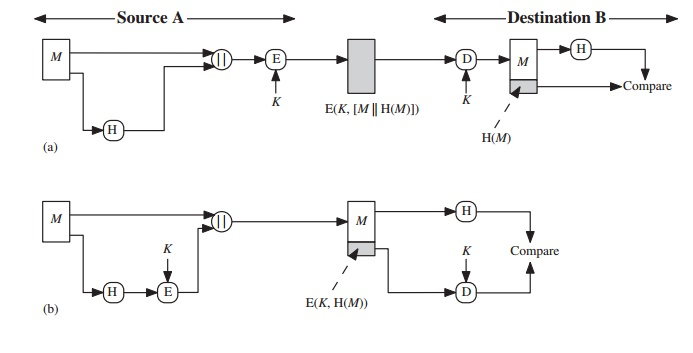
\includegraphics[width=\textwidth]{img/alice.jpg}
    \caption{Utilizzo delle hash function per l'autenticazione dei messaggi}
    \label{fig:itm}
\end{figure}

\paragraph{Firma digitale}
Un'applicazione strettamente correlata all'\textit{autenticazione dei messaggi} è la \textit{firma digitale}. Il funzionamento della firma digitale è simile a quello del MAC. Nella firma digitale, il valore hash di un messaggio viene cifrato con la chiave privata di un utente. Chiunque conosca la chiave pubblica dell'utente può verificare l'integrità del messaggio associato alla firma digitale. In questo contesto, un attaccante che volesse alterare il messaggio avrebbe bisogno di conoscere la chiave privata dell'utente.

\begin{figure}[H]
    \centering
    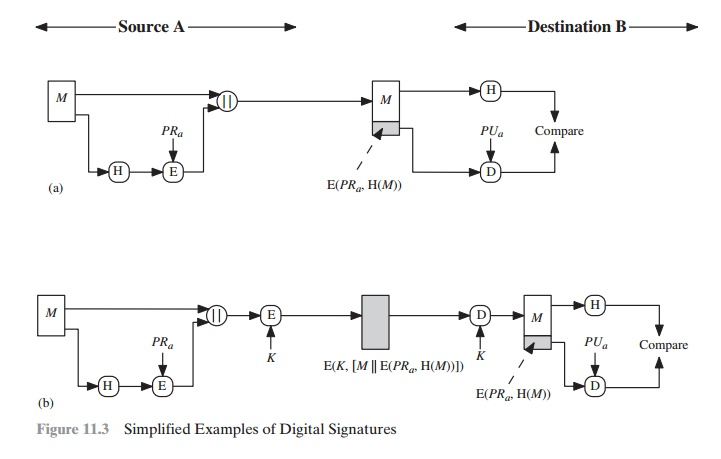
\includegraphics[width=\textwidth]{img/digital.jpg}
    \caption{Esempio di firma digitale}
    \label{fig:itm}
\end{figure}


La Figura 3 mostra, in modo semplificato, come un codice hash viene utilizzato per fornire una firma digitale.

\begin{itemize}
    \item[a.] Il codice hash viene cifrato utilizzando la crittografia a chiave pubblica con la chiave privata del mittente. Fornisce anche una firma digitale, perché solo il mittente avrebbe potuto produrre il codice hash cifrato. Questa è, in realtà, l'essenza della tecnica della firma digitale.
    \item[b.] Se si desidera la riservatezza oltre alla firma digitale, il messaggio più il codice hash cifrato con la chiave privata possono essere cifrati usando una chiave segreta simmetrica. Questa è una tecnica comune.
\end{itemize}

\paragraph{Proprietà di base}
Per facilitare ulteriori definizioni, sono elencate tre potenziali proprietà (in aggiunta alla facilità di calcolo e compressione come per la Definizione 9.1), per una funzione hash non chiavata \( h \) con input \( x, x' \) e output \( y, y' \).

\begin{enumerate}
    \item \textbf{Resistenza alla Pre-Immagine} --- per praticamente tutti gli output pre-specificati, è computazionalmente infattibile trovare un input che ha come hash tale output, ovvero, trovare una pre-immagine \( x' \) tale che \( h(x') = y \) quando è dato un \( y \) per il quale un input corrispondente non è noto.
    \item \textbf{Resistenza alla Seconda Pre-Immagine} --- è computazionalmente infattibile trovare un secondo input che ha lo stesso output di un input specificato, ovvero, dato \( x \), trovare una seconda pre-immagine \( x' \neq x \) tale che \( h(x) = h(x') \).
    \item \textbf{Resistenza alle Collisioni} --- è computazionalmente infattibile trovare due input distinti \( x, x' \) che hanno come hash lo stesso output, ovvero, tali che \( h(x) = h(x') \). (Notare che qui c'è la libera scelta di entrambi gli input.)
\end{enumerate}

I termini ``facile'' e ``computazionalmente infattibile'' (o ``difficile'') sono intenzionalmente lasciati senza una definizione formale; si intende che siano interpretati relativamente a un quadro di riferimento compreso. ``Facile'' potrebbe significare tempo e spazio polinomiali; o più praticamente, entro un certo numero di operazioni di macchina o unità di tempo – forse secondi o millisecondi. Una definizione più specifica di ``computazionalmente infattibile'' potrebbe coinvolgere uno sforzo super-polinomiale; richiedere uno sforzo ben superiore alle risorse comprese; specificare un limite inferiore sul numero di operazioni o sulla memoria richiesta in termini di un parametro di sicurezza specificato; o specificare che la probabilità che una proprietà sia violata sia esponenzialmente piccola.

\subsubsection{Accordo di chiave basato su tecniche asimmetriche}%CAP 12 LIBRO CRITTOGRAPHY

L'accordo di chiave Diffie-Hellman (chiamato anche scambio di chiavi esponenziale) è una tecnica fondamentale che fornisce un accordo di chiave non autenticato. Questa sezione discute i protocolli di stabilimento chiave basati su scambio di chiavi esponenziale, nonché il concetto di chiavi pubbliche implicitamente certificate e il loro utilizzo nei protocolli Diffie-Hellman.

\paragraph{Diffie-Hellman e protocolli di accordo di chiave correlati}

Questa sezione considera il protocollo Diffie-Hellman di base e i protocolli correlati che forniscono varie garanzie di autenticazione.

\paragraph{Accordo di chiave Diffie-Hellman}
L'accordo di chiave Diffie-Hellman ha fornito la prima soluzione pratica al problema della distribuzione delle chiavi, permettendo a due parti, che non si sono mai incontrate in precedenza o condiviso materiale di chiavi, di stabilire un segreto condiviso scambiando messaggi su un canale aperto. La sicurezza si basa sull'intrattabilità del problema Diffie-Hellman e sul problema correlato del calcolo dei logaritmi discreti. La versione di base fornisce protezione sotto forma di segretezza della chiave risultante da avversari passivi (intercettatori), ma non da avversari attivi in grado di intercettare, modificare o iniettare messaggi. Nessuna delle parti ha garanzie sull'identità della fonte del messaggio in entrata o sull'identità della parte che potrebbe conoscere la chiave risultante, cioè autenticazione dell'entità o autenticazione della chiave.

\begin{mdframed}
\begin{center}
    \vspace{10pt}
    \textbf{Accordo di chiave Diffie-Hellman (versione base)} \\
    Sommario: A e B inviano reciprocamente un messaggio su un canale aperto. \\
   Risultato: segreto condiviso \( K \) noto sia a A che a B.
    \vspace{10pt}
\end{center} 

\begin{enumerate}
    \item \textbf{Configurazione iniziale.} Viene scelto e pubblicato un primo appropriato \( p \) e un generatore \( \alpha \) di \( Z^*_p \) con \( 2 \leq \alpha \leq p - 2 \).
    
    \item \(A\) invia a \(B\)
    \begin{equation}\tag{1}\label{eq:protocol_msg_1}
        y = \alpha^x \mod p
    \end{equation}
    che rappresenta la potenza di \( \alpha \) elevata al valore segreto \( x \) modulo \( p \).
    
    \(B\) invia a \(A\)
    \begin{equation}\tag{2}\label{eq:protocol_msg_2}
        z = \alpha^y \mod p
    \end{equation}
    che rappresenta la potenza di \( \alpha \) elevata al valore segreto \( y \) modulo \( p \).
    
    \item \textbf{Azioni del protocollo.} Eseguire i seguenti passaggi ogni volta che è richiesta una chiave condivisa.
    \begin{enumerate}
        \item A sceglie un segreto casuale \( x \), con \( 1 \leq x \leq p - 2 \), e invia a B il messaggio (1).
        \item B sceglie un segreto casuale \( y \), con \( 1 \leq y \leq p - 2 \), e invia a A il messaggio (2).
        \item B riceve \( y \) (cioè \( \alpha^x \)) e calcola la chiave condivisa come \( K = y^y \mod p \).
        \item A riceve \( z \) (cioè \( \alpha^y \)) e calcola la chiave condivisa come \( K = z^x \mod p \).
    \end{enumerate}
\end{enumerate}
\end{mdframed}

%\begin{figure}[H]
  %  \centering
    %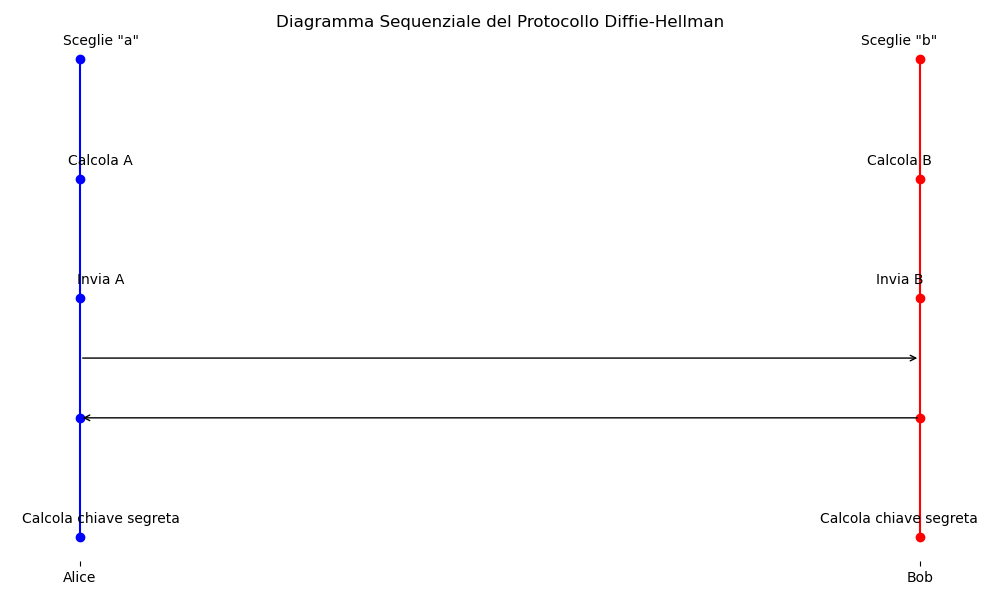
\includegraphics[width=\textwidth]{img/diagrSquDH.png}
  %  \caption{Interactive Turing Machine.}
  %  \label{fig:itm}
%\end{figure}

%%Una versione alternativa del Protocollo di Diffie-Hellman offre autenticazione mutua delle chiavi. Poniamo \( \alpha^x \) e \( \alpha^y \mod p \) come chiavi pubbliche a lungo termine delle parti rispettive. Distribuiamo queste chiavi utilizzando certificati firmati, definendo quindi la chiave condivisa a lungo termine per questo paio di utenti come \( K = \alpha^{xy} \). Se tali certificati sono disponibili in anticipo, non è necessario scambiare messaggi crittografici. Tuttavia, la natura invariante di questa chiave \( K \) è uno svantaggio. Una soluzione potrebbe coinvolgere l'uso di tecniche di aggiornamento della chiave.



\subsection{Architettura}
%DOCUMENTO SSL WL040C-21.tex
SSL è composto da quattro protocolli. Tre dei quattro, il Protocollo di Handshake SSL, il Protocollo di Cambio Cifra SSL e il Protocollo di Allerta SSL, vengono utilizzati per configurare e gestire canali di comunicazione sicuri. Il protocollo rimanente, il Protocollo di Record SSL, fornisce il servizio di sicurezza richiesto dalle applicazioni. L'SSL si trova tra il livello applicativo e il livello TCP dei protocolli TCP/IP. Una volta che è stato stabilito un canale sicuro, l'SSL prende i messaggi da trasmettere, frammenta il messaggio in blocchi gestibili, comprime opzionalmente i dati, applica un codice di autenticazione del messaggio (MAC), cifra, prefissa l'intestazione del record SSL e invia il risultato al livello TCP. In ultima analisi, questi blocchi di dati vengono ricevuti e i dati vengono decifrati, verificati, decompressi, riassemblati nel livello SSL del ricevitore e quindi consegnati ai clienti di livello superiore.
Ci sono molte altre eccellenti fonti secondarie che forniscono ulteriori informazioni di base oltre alle specifiche dei protocolli. I protocolli utilizzati per stabilire un canale sicuro danno a SSL la sua flessibilità per la comunicazione client/server.

SSL è flessibile nella scelta di quali algoritmi di cifratura simmetrica, digest del messaggio e di autenticazione possono essere utilizzati. Quando un client SSL prende contatto con un server SSL, concordano sui metodi di cifratura più forti che hanno in comune. Inoltre, SSL fornisce una compressione dei dati integrata. La compressione dei dati deve essere effettuata prima della cifratura.

Quando viene stabilita una connessione SSL, le comunicazioni da browser a server e da server a browser sono cifrate. La cifratura include:
\begin{itemize}
    \item URL del documento richiesto
    \item Contenuti del documento
    \item Contenuti dei moduli del browser
    \item Cookies inviati dal browser al server
    \item Cookies inviati dal server al browser
    \item Contenuti dell'intestazione HTTP, ma non da un particolare browser a un particolare server.
\end{itemize}

In particolare, gli indirizzi socket, l'ndirizzo IP e il numero di porta non sono cifrati; tuttavia, può essere utilizzato un server proxy se è richiesto questo tipo di privacy.

\begin{figure}[htbp]
\centering
\begin{tikzpicture}[block/.style={rectangle, draw, text width=2cm, align=center, minimum height=1cm, outer sep=0pt},
                    bigblock/.style={rectangle, draw, text width=8.5cm, align=center, minimum height=1cm, outer sep=0pt},
                    node distance=0.5cm]

% Place the small blocks
\node[block] (handshake) {SSL Handshake};
\node[block, right=of handshake] (change) {SSL Change\\ Cipher Spec};
\node[block, right=of change] (alert) {SSL Alert};
\node[block, right=of alert] (http) {HTTP/FTP};

% Position the large block slightly to the right of the small blocks
\node[bigblock, below=0.5cm of handshake.south, xshift=4cm] (record) {SSL Record};
\node[bigblock, below=of record] (tcpip) {TCP/IP};

\end{tikzpicture}
\caption{Struttura a livelli del protocollo SSL}
\end{figure}

\subsubsection{Struttura dei messaggi SSL}
La struttura dei messaggi in SSL (Secure Socket Layer) è piuttosto complessa e si basa su vari protocolli che operano insieme per fornire una comunicazione sicura. SSL è stato il predecessore di TLS (Transport Layer Security), che è la versione attualmente utilizzata e migliorata. La struttura dei messaggi è simile tra SSL e TLS, anche se ci sono alcune differenze nelle versioni più recenti di TLS.

Ecco un'analisi generale di come sono strutturati i messaggi in SSL.
\begin{enumerate}
    \item \textbf{Protocollo Record}:
    \begin{itemize}
        \item Questo protocollo definisce la struttura di base di tutti i messaggi trasmessi tra client e server.
        \item I messaggi possono essere compressi, cifrati e muniti di un MAC (Message Authentication Code) per garantire integrità e autenticità.
        \item Ogni messaggio ha un'intestazione che indica il tipo di messaggio (ad es. handshake, alert, change cipher spec, application data).
    \end{itemize}

    \item \textbf{Protocollo Handshake}:
    \begin{itemize}
        \item Questo protocollo è responsabile della negoziazione dei parametri di sicurezza tra client e server.
        \item I messaggi di questo protocollo includono: \texttt{ClientHello}, \texttt{ServerHello}, \texttt{Certificate}, \texttt{ServerKeyExchange}, \texttt{ClientKeyExchange}, ecc.
    \end{itemize}

    \item \textbf{Protocollo Alert}:
    \begin{itemize}
        \item Utilizzato per trasmettere messaggi di avviso o errore.
        \item Ad esempio, se si verifica un errore durante l'handshake, verrà inviato un messaggio di alert.
    \end{itemize}

    \item \textbf{Protocollo Change Cipher Spec}:
    \begin{itemize}
        \item Comprende un singolo messaggio che indica al destinatario di cambiare l'algoritmo di cifratura utilizzato.
    \end{itemize}

    \item \textbf{Applicazione Data Protocol}:
    \begin{itemize}
        \item Trasporta i dati dell'applicazione, che sono stati cifrati e protetti come definito dai parametri di sicurezza concordati.
    \end{itemize}
\end{enumerate}

Parleremo poi più approfonditamente di questi protocolli nel capitolo \ref{protocolli}




\subsubsection{Protocolli utilizzati}\label{protocolli}
\paragraph{Record protocol}
\begin{quote}
Il protocollo SSL Record funziona come base per altri tre protocolli e fornisce confidenzialità e integrità ai messaggi dei livelli superiori. Sul lato mittente, segmenta le informazioni in diversi blocchi, li comprime, calcola il MAC e cripta i blocchi insieme al corrispondente MAC. Sul lato destinatario, questi processi vengono eseguiti in direzione opposta prima che i messaggi originali vengano consegnati al destinatario. Per impostazione predefinita, la compressione è disabilitata in SSLv3.0 e in tutte le versioni di TLS. La struttura di flusso della creazione dei pacchetti SSL è divisa in cinque parti:

\begin{enumerate}
    \item \textbf{Algoritmi di Compressione:} Le tecniche di compressione lossless vengono chiamate dal protocollo record SSL per comprimere i dati senza alcuna perdita. (ad esempio, codifica Huffman, LZ77, GZIP, ecc.)
    \item \textbf{Algoritmi Hash:} Le funzioni hash sicure svolgono un ruolo importante per garantire la confidenzialità di ogni segmento di dati. Gli algoritmi più popolari come MD5 e SHA sono utilizzati per calcolare il MAC. (ad esempio, MD5, SHA-1, SHA-224, SHA-256, ecc.)
    \item \textbf{Algoritmi di Crittografia:} Tecniche di cifratura simmetrica a flusso o a blocchi vengono utilizzate per creare il payload SSL. Nel caso della cifratura a flusso, il blocco compresso e il MAC vengono criptati insieme. Bit di padding vengono aggiunti insieme al MAC al blocco prima della cifratura a blocchi.
    \item \textbf{Aggiunta dell'Header SSL:} Ogni unità di dati criptata viene dotata di un'intestazione specifica del protocollo SSL, che include informazioni come il tipo di contenuto, la versione del protocollo e la lunghezza del blocco.
    \item \textbf{Trasmissione via TCP/IP:} I dati processati vengono infine inviati al livello di rete, tipicamente usando il protocollo TCP/IP, per la trasmissione al destinatario. \cite{sslprot}
\end{enumerate}
\end{quote}

%Il Protocollo SSL Record fornisce due dei tre requisiti essenziali per la trasmissione sicura dei dati: riservatezza e integrità del messaggio. La riservatezza è fornita dalla cifratura simmetrica che utilizza la chiave di sessione condivisa scambiata tra il client e il server durante il protocollo di handshake. Questo protocollo di handshake definisce anche una chiave segreta condivisa che può essere utilizzata per creare un codice di autenticazione del messaggio (MAC), che può essere utilizzato per garantire l'integrità del messaggio. Il terzo requisito, l'autenticazione, è fornito dal protocollo di handshake nella sua richiesta di almeno un certificato del server.

%Il protocollo di record elabora un messaggio innanzitutto suddividendolo in frammenti di dimensione fissa uguale, riempiendo l'ultimo frammento se necessario. Il passaggio successivo è la compressione facoltativa di ogni frammento. Una volta completata la compressione, viene calcolato un MAC per ogni frammento e aggiunto al frammento. Il risultato viene quindi cifrato utilizzando la chiave e l'algoritmo concordato tra il client e il server. Viene aggiunto un'intestazione di record SSL. Quindi, questo segmento viene passato al livello TCP per l'elaborazione. I dati ricevuti vengono elaborati dal protocollo ricevente nel processo inverso: i dati vengono decifrati, verificati tramite il MAC e decompressi se necessario, i frammenti vengono riassemblati e il risultato viene quindi inviato all'applicazione di destinazione.

\paragraph{Handshake protocol} %PRESO DAL DOCUMENTO SSL
Tra i quattro protocolli che compongono SSL e TLS, il protocollo di handshake è il più critico. Questo protocollo è responsabile dell'instaurazione della connessione, poichè utilizza una sequenza di messaggi che permettono al client e al server di autenticarsi reciprocamente e di concordare gli algoritmi di cifratura e MAC, nonché le relative chiavi. 

Il campo "type" del protocollo di handshake indica uno dei 10 messaggi elencati nella Tabella 1 sottostante. "Length" è la lunghezza del messaggio in byte. "Content" sono i parametri associati al tipo di messaggio (vedi Tabella 1).

Il passo 1 è rappresentato dal messaggio \textit{ClientHello}. I suoi parametri sono:
\begin{itemize}
    \item \textbf{versione}: La versione del protocollo SSL che il client desidera utilizzare durante questa sessione. Dovrebbe essere la versione più recente supportata dal client.
    \item \textbf{random}: Una struttura casuale generata dal client. Ha una lunghezza di 32 byte. I primi quattro byte rappresentano l'orario di generazione del messaggio e i restanti 28 byte sono generati utilizzando un generatore di numeri casuali sicuro. Questo valore verrà utilizzato come input per la generazione della chiave. Il timestamp previene possibili attacchi di tipo \textit{man-in-the-middle}.
    \item \textbf{session id}: L'ID di una sessione che il client desidera utilizzare per questa connessione sarà vuoto se non è disponibile alcun \textit{session id} o se il client desidera generare nuovi parametri di sicurezza.
    \item \textbf{cipher suites}: Una lista delle opzioni crittografiche supportate dal client, ordinate in base alle preferenze. Se il campo session id non è vuoto, questa lista deve includere almeno la cipher suite di quella sessione.
    \item \textbf{compression methods}: Una lista dei metodi di compressione supportati dal client, ordinati per preferenza. Questa lista deve sempre includere il metodo di compressione nullo. 
\end{itemize}

Dopo aver inviato il messaggio \textit{ClientHello}, il client attende un messaggio \textit{ServerHello}. Qualsiasi altro messaggio di handshake restituito dal server, ad eccezione di una richiesta di hello, è considerato un errore fatale.

Il passo 2 rappresenta il messaggio \textit{ServerHello}. I parametri di questo messaggio sono:
\begin{itemize}
    \item \textbf{server version}: Questo campo conterrà il minore tra quello suggerito dal client nel messaggio \textit{ClientHello} e il più elevato supportato dal server.
    \item \textbf{random}: Questa struttura è generata dal server e deve essere diversa da quella del \textit{ClientHello}.
    \item \textbf{session id}: È l'identità della sessione corrispondente a questa connessione.
    \item \textbf{cipher suite}: La singola cipher suite selezionata dal server dalla lista nel campo cipher suites del messaggio \textit{ClientHello}.
    \item \textbf{compression method}: L'algoritmo di compressione selezionato dal server dalla lista nel campo compression methods del messaggio \textit{ClientHello}.
\end{itemize}

Il \textbf{Passo 3} riguarda il messaggio \textit{Certificate}. Se il server deve essere autenticato (quasi sempre il caso), il server invia il proprio certificato subito dopo il messaggio \textit{ServerHello}. Il tipo di certificato deve essere adatto all'algoritmo di scambio chiavi della suite cifrante selezionata, ed è generalmente un certificato X.509.v3. Lo stesso tipo di messaggio viene utilizzato anche per la risposta del client al messaggio \textit{CertificateRequest} del server. Se il server non ha un certificato o se viene utilizzata una tecnica di scambio chiavi diversa da RSA o Diffie-Hellman, il server invierà il messaggio \textit{ServerKeyExchange}.

Il \textbf{Passo 4} (opzionale) permette a un server non anonimo di richiedere facoltativamente un certificato al client, se appropriato per la suite cifrante selezionata. Il messaggio \textit{CertificateRequest} ha due parametri:
\begin{itemize}
    \item \textbf{types}: Una lista dei tipi di certificati richiesti, ordinati secondo le preferenze del server.
    \item \textbf{authorities}: Una lista dei nomi distintivi delle autorità certificatrici accettabili.
\end{itemize}

Dopo il \textbf{Passo 3} (o il \textbf{Passo 4} opzionale), il server invierà un messaggio \textit{ServerHelloDone}, indicando che ha inviato tutti i messaggi di handshake necessari per la fase di saluto del server. Il client, dopo aver ricevuto questo messaggio, controllerà la validità del certificato del server e l'accettabilità dei parametri del messaggio \textit{ServerHello}.

Il \textbf{Passo 5} (opzionale) concerne il messaggio \textit{Certificate}. Questo messaggio viene inviato dal client solo se il server richiede un certificato. Se non è disponibile un certificato appropriato, il client dovrebbe inviare un avviso \textit{NoCertificate}.

Nel \textbf{Passo 6}, abbiamo il messaggio \textit{ClientKeyExchange}. Il contenuto del messaggio dipende dal tipo di scambio chiavi concordato durante la prima fase del processo di handshake. Il metodo di scambio delle chiavi è determinato dalla suite cifrante selezionata e dal tipo di certificato del server. Ad esempio, se il client e il server concordano sul metodo di scambio chiavi RSA, il client genera un segreto \textit{premaster} di 48 byte e lo cifra con la chiave pubblica del certificato del server o utilizza la chiave pubblica temporanea dal messaggio \textit{ServerKeyExchange} del server.

Se il server ha richiesto un certificato client e necessita di verifica, il client invierà un messaggio \textit{CertificateVerify} per fornire una verifica esplicita del suo certificato client.

Al \textbf{Passo 8}, il client invia un messaggio \textit{ChangeCipherSpec} indicando che è passato alla suite cifrante concordata. Tutti i messaggi successivi saranno inviati utilizzando gli algoritmi di cifratura concordati e le relative chiavi. È importante notare che il messaggio \textit{ChangeCipherSpec} è un protocollo separato e non fa parte del protocollo di Handshake. Questo serve a rendere SSL e TLS più efficienti. Il messaggio \textit{ChangeCipherSpec} consiste in un solo byte.

Nel \textbf{Passo 9}, il client invia il messaggio di handshake \textit{Finish}. Il messaggio è una concatenazione di due valori di digest del messaggio. Ogni valore viene calcolato utilizzando un diverso algoritmo di digest del messaggio - MD5 e SHA - sui medesimi dati. I dati sono il segreto principale e l'insieme dei messaggi di handshake inviati fino a quel momento.

In risposta a questi due messaggi client, il server invia la sua versione del messaggio \textit{ChangeCipherSpec} e un messaggio \textit{Finished} calcolato utilizzando gli stessi dati del client. Se il valore di questo messaggio \textit{Finished} differisce dal valore del messaggio \textit{Finished} inviato dal client, ciò indica che l'handshake è stato modificato e potrebbe non essere stata stabilita una connessione sicura. Quando il client riceve il messaggio \textit{Finish} dal server, lo confronta con il valore del messaggio \textit{Finish} calcolato localmente. Se corrispondono, tutto è in ordine; altrimenti, potrebbe non essere stata stabilita una connessione sicura.

\paragraph{Change Cipher Spec Protocol}
Il protocollo \textit{Change Cipher Spec (CCS)} svolge un ruolo fondamentale nella comunicazione SSL (Secure Sockets Layer), agendo come indicatore di transizione tra la fase di negoziazione e la fase di scambio sicuro dei dati. Nonostante la sua semplicità, essendo composto da un unico messaggio di un solo byte con valore 1, il protocollo CCS è essenziale per garantire la sicurezza e l'integrità della comunicazione.

Durante la fase di handshake in una sessione SSL, le parti coinvolte (client e server) negoziano e concordano sugli algoritmi crittografici da utilizzare, quali algoritmi di cifratura, hash e autenticazione. Tuttavia, le nuove configurazioni concordate non vengono applicate immediatamente. Il protocollo Change Cipher Spec entra in gioco in questo momento: una volta ricevuto il messaggio CCS, entrambe le parti sono informate che devono iniziare ad utilizzare le nuove configurazioni crittografiche concordate per proteggere la comunicazione.

Inoltre, il protocollo CCS funge anche da meccanismo di conferma e sincronizzazione tra le parti, assicurando che entrambe procedano coerentemente attraverso le fasi del protocollo SSL. Ricevere il messaggio CCS assicura che le comunicazioni successive siano protette utilizzando i nuovi parametri e algoritmi crittografici, garantendo che la sessione continui con una sicurezza e integrità rinnovate e robuste. \cite{sslarchitecture}

\begin{figure}[H]
    \centering
    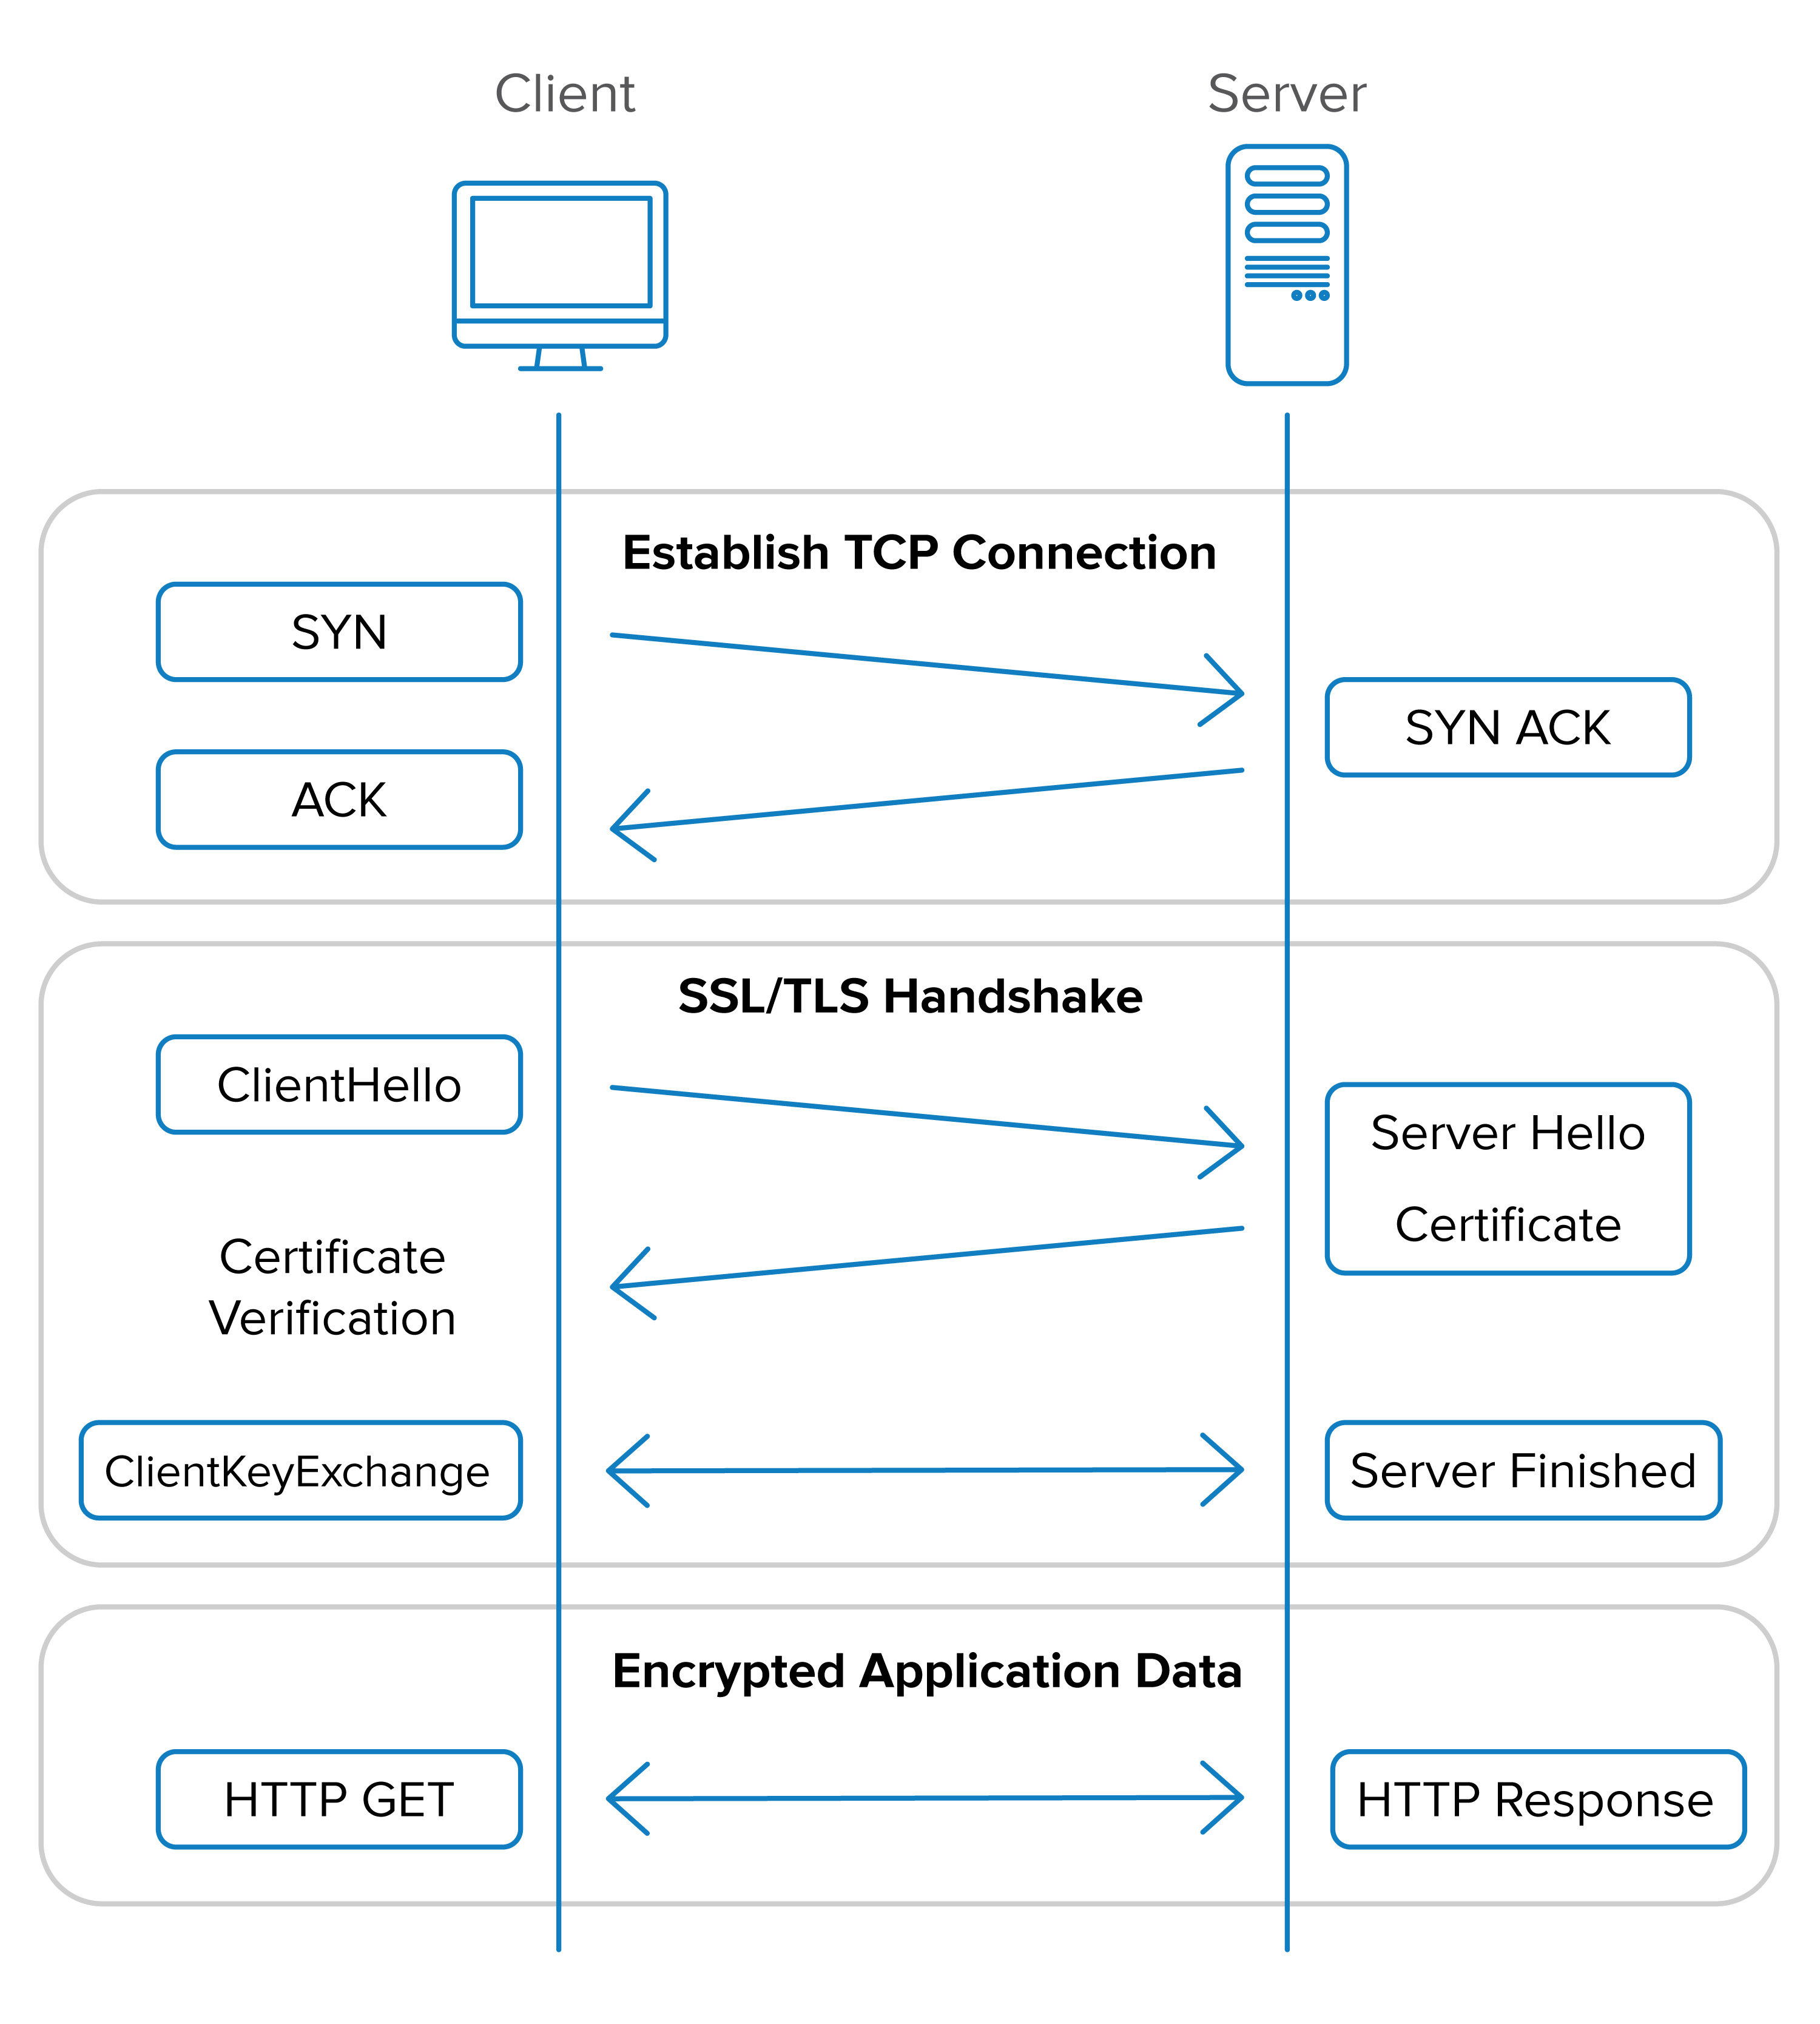
\includegraphics[width=\textwidth]{img/handshake.png}
    \caption{Esempio di firma digitale}
    \label{fig:itm}
\end{figure}

\subsection{Protocollo HTTPS}
HTTPS (HTTP su SSL) si riferisce alla combinazione di HTTP e SSL per implementare una comunicazione sicura tra un browser Web e un server Web. La funzionalità HTTPS è integrata in tutti i browser Web moderni. Il suo utilizzo dipende dal supporto del server Web alla comunicazione HTTPS. Ad esempio, alcuni motori di ricerca non supportano HTTPS.

La principale differenza percepita da un utente di un browser Web è che gli indirizzi URL (Uniform Resource Locator) iniziano con \texttt{https://} invece che \texttt{http://}. Una normale connessione HTTP utilizza la porta 80. Se viene specificato HTTPS, viene utilizzata la porta 443, che invoca SSL.

Quando si utilizza HTTPS, i seguenti elementi della comunicazione vengono criptati:
\begin{itemize}
    \item URL del documento richiesto
    \item Contenuto del documento
    \item Contenuti dei moduli del browser (compilati dall'utente del browser)
    \item Cookie inviati dal browser al server e dal server al browser
    \item Contenuti dell'intestazione HTTP
\end{itemize}

HTTPS è documentato in RFC 2818, HTTP su TLS. Non ci sono cambiamenti fondamentali nell'uso di HTTP su SSL o TLS, e entrambe le implementazioni vengono chiamate HTTPS.

\paragraph{Inizio connessione}
Per HTTPS, l'agente che funge da client HTTP agisce anche come client TLS. Il client inizia una connessione al server sulla porta appropriata e poi invia il ClientHello di TLS per iniziare la stretta di mano di TLS. Quando la stretta di mano di TLS è terminata, il client può poi iniziare la prima richiesta HTTP. Tutti i dati HTTP devono essere inviati come dati applicativi TLS. Dovrebbe essere seguito il comportamento HTTP normale, incluso il mantenimento delle connessioni.

Ci sono tre livelli di consapevolezza di una connessione in HTTPS:
\begin{itemize}
    \item Al livello HTTP, un client HTTP richiede una connessione a un server HTTP inviando una richiesta di connessione al livello inferiore successivo. Tipicamente, il livello successivo più basso è TCP, ma può anche essere TLS/SSL.
    \item Al livello di TLS, viene stabilita una sessione tra un client TLS e un server TLS. Questa sessione può supportare una o più connessioni in qualsiasi momento.
    \item Una richiesta TLS per stabilire una connessione inizia con l'instaurazione di una connessione TCP tra l'entità TCP sul lato client e l'entità TCP sul lato server.
\end{itemize}

\paragraph{Chiusura connessione}
Un client HTTP o un server può indicare la chiusura di una connessione includendo la seguente riga in un record HTTP: \texttt{Connection: close}. Questo indica che la connessione verrà chiusa dopo la consegna di questo record.

La chiusura di una connessione HTTPS richiede che TLS chiuda la connessione con l'entità TLS peer sul lato remoto, che comporterà la chiusura della connessione TCP sottostante. Al livello TLS, il modo corretto per chiudere una connessione è per ogni lato utilizzare il protocollo di allerta TLS per inviare un allarme \texttt{close\_notify}. Le implementazioni TLS devono iniziare uno scambio di allarmi di chiusura prima di chiudere una connessione.

I clienti HTTP devono anche essere in grado di affrontare una situazione in cui la connessione TCP sottostante viene terminata senza un allarme \texttt{close\_notify} precedente e senza un indicatore \texttt{Connection: close}. Tale situazione potrebbe essere dovuta a un errore di programmazione sul server o a un errore di comunicazione che fa cadere la connessione TCP. Tuttavia, la chiusura TCP non annunciata potrebbe essere la prova di qualche tipo di attacco. Quindi il client HTTPS dovrebbe emettere un tipo di avviso di sicurezza quando ciò si verifica.


\section{Evoluzione da SSL a TSL}

\subsection{Storia}
%VERSIONE 1
Il protocollo SSL fu sviluppato da Netscape, all'epoca in cui Netscape Navigator dominava Internet. La prima versione del protocollo non vide mai la luce del giorno, ma la successiva, la versione 2, fu rilasciata nel novembre 1994. La prima implementazione fu in Netscape Navigator 1.1, che fu rilasciato nel marzo 1995.

Sviluppato con poca o nessuna consultazione con esperti di sicurezza esterni a Netscape, SSL 2 si rivelò un protocollo scadente con gravi debolezze. Questo costrinse Netscape a lavorare su SSL 3, che fu rilasciato alla fine del 1995. Nonostante condividesse il nome con le versioni precedenti del protocollo, SSL 3 era un design di protocollo completamente nuovo che stabilì il design che conosciamo oggi.

Nel maggio 1996, fu formato il gruppo di lavoro TLS per migrare SSL da Netscape a IETF. Il processo fu dolorosamente lento a causa delle lotte politiche tra Microsoft e Netscape, una conseguenza della lotta più grande per dominare il Web. TLS 1.0 fu finalmente rilasciato nel gennaio 1999, come RFC 2246. Anche se le differenze rispetto a SSL 3 non erano grandi, il nome fu cambiato per accontentare Microsoft.

La versione successiva, TLS 1.1, non fu rilasciata fino all'aprile 2006 e conteneva essenzialmente solo correzioni di sicurezza. Tuttavia, una modifica importante al protocollo fu l'incorporazione delle estensioni TLS, che furono rilasciate un paio di anni prima, nel giugno 2003.

TLS 1.2 fu rilasciato nell'agosto 2008. Ha aggiunto il supporto per la crittografia autenticata e in generale ha rimosso tutti i primitivi di sicurezza hard-coded dalla specifica, rendendo il protocollo completamente flessibile.

La versione successiva del protocollo, attualmente in sviluppo, si sta configurando come una revisione importante volta a semplificare il design, rimuovendo molte delle caratteristiche più deboli e meno desiderabili, e migliorando le prestazioni. È possibile seguire le discussioni sulla mailing list del gruppo di lavoro TLS.

%VERSIONE2
Oggi nel mondo degli affari, il World Wide Web (WWW) rappresenta il modello di riferimento dietro ogni azione. Con l'aumento della domanda, c'è una necessità di trasformazione dai servizi web ai servizi web sicuri. I protocolli Secure Socket Layer (SSL)/Transport Layer Security (TLS) sono utilizzati per fornire servizi affidabili sul protocollo di trasporto. SSL ha subito diversi aggiornamenti, come SSLv1.0, SSLv2.0 e SSLv3.0. La versione SSLv3.1 è essenzialmente chiamata TLSv1.0, che offre compatibilità retroattiva con le versioni precedenti di SSL. Il protocollo SSL funziona su due livelli di servizio, il primo è la connessione SSL e il secondo è la sessione SSL. La connessione SSL funziona a livello di trasporto per stabilire collegamenti tra client e server. Le associazioni peer-to-peer consentono di creare sessioni che sono effimere. Ogni sessione SSL è associata a una singola connessione SSL. Il protocollo di stretta di mano SSL/TLS viene utilizzato per creare sessioni scambiando vari parametri (ad es., numeri casuali, ID di sessione, suite di cifratura, tecniche di compressione, ecc.). Ogni sessione è gestita da due stati principali. Lo stato della sessione comprende vari parametri come l'identificatore di sessione, il certificato X509, tecniche di compressione, specifiche di cifratura, segreto principale, ecc. D'altro canto, i parametri di stato di connessione comprendono segreti MAC di invio del server e del client, vettori di inizializzazione, numeri di sequenza, ecc.

\subsection{Introduzione a TSL}
Il Protocollo Record di SSL fornisce servizi di sicurezza di base a vari protocolli di livello superiore. In particolare, l'Hypertext Transfer Protocol (HTTP), che fornisce il servizio di trasferimento per l'interazione client/server Web, può operare sopra SSL.
SSL è composto da quattro protocolli. Tre dei quattro, il Protocollo di Handshake SSL, il Protocollo di Change Cipher Spec SSL e il Protocollo Alert SSL, sono utilizzati per impostare e gestire canali di comunicazione sicuri. Il protocollo rimanente, il Protocollo di Registrazione SSL, fornisce il servizio di sicurezza richiesto dalle applicazioni. SSL si trova tra il livello applicativo e il livello TCP dei protocolli TCP/IP.

Due importanti concetti di TLS sono la sessione SSL e la connessione SSL, che sono definiti nella specifica come segue:
\begin{itemize}
    \item \textbf{Connessione:} Una connessione è un trasporto (nella definizione del modello di stratificazione OSI) che fornisce un tipo appropriato di servizio. Per SSL, tali connessioni sono relazioni peer-to-peer. Le connessioni sono transitorie. Ogni connessione è associata a una sessione.
    \item \textbf{Sessione:} Una sessione SSL è un'associazione tra un client e un server. Le sessioni sono create dal Protocollo Handshake. Le sessioni definiscono un insieme di parametri di sicurezza crittografici, che possono essere condivisi tra molteplici connessioni. Le sessioni sono utilizzate per evitare la costosa negoziazione di nuovi parametri di sicurezza per ogni connessione.
\end{itemize}
Tra qualsiasi coppia di parti (applicazioni come HTTP su client e server), possono esistere molteplici connessioni sicure. In teoria, potrebbero anche esistere molteplici sessioni simultanee tra le parti, ma questa funzionalità non viene utilizzata nella pratica.

Ci sono vari stati associati ad ogni sessione. Una volta che una sessione è stabilita, esiste uno stato operativo corrente sia per la lettura che per la scrittura (cioè, ricezione e invio). Inoltre, durante il Protocollo di Handshake, vengono creati stati di lettura e scrittura pendenti. Al termine con successo del Protocollo di Handshake, gli stati pendenti diventano gli stati correnti.

\subsubsection{Protocollo record TLS}
Il Protocollo di Record SSL fornisce due servizi per le connessioni di questo tipo:

\begin{itemize}
    \item \textbf{Confidenzialità:} Il Protocollo di Handshake definisce una chiave segreta condivisa che viene utilizzata per la cifratura convenzionale dei carichi utili SSL.
    \item \textbf{Integrità del messaggio:} Il Protocollo di Handshake definisce anche una chiave segreta condivisa che viene utilizzata per formare un codice di autenticazione del messaggio (MAC).
\end{itemize}

Il Protocollo di Record prende un messaggio dell'applicazione da trasmettere, frammenta i dati in blocchi gestibili, comprime opzionalmente i dati, applica un MAC, cifra, aggiunge un'intestazione, e trasmette l'unità risultante in un segmento TCP. I dati ricevuti vengono decifrati, verificati, decompressi e riassemblati prima di essere consegnati agli utenti di livello superiore.

Il primo passo è la frammentazione. Ogni messaggio del livello superiore viene frammentato in blocchi di \(2^{14}\) byte (16.384 byte) o meno. Successivamente, la compressione viene applicata opzionalmente. La compressione deve essere senza perdita e non può aumentare la lunghezza del contenuto di più di 1024 byte. In TLSv2, non viene specificato alcun algoritmo di compressione, quindi l'algoritmo di compressione predefinito è nullo.

Il passo successivo nella lavorazione è calcolare un codice di autenticazione del messaggio sui dati compressi. TLS utilizza l'algoritmo HMAC definito nella RFC 2104. Ricordiamo dal Capitolo 3 che HMAC è definito come:

\[ \text{HMAC}(M) = H[(K^+ \oplus \text{opad}) \Vert H[(K^+ \oplus \text{ipad}) \Vert M]] \]
dove:
\begin{itemize}
    \item \( H \) = funzione hash incorporata (per TLS, MD5 o SHA-1)
    \item \( M \) = messaggio in input a HMAC
    \item \( K^+ \) = chiave segreta imbottita con zeri a sinistra in modo che il risultato sia uguale alla lunghezza del blocco del codice hash (per MD5 e SHA-1, lunghezza blocco = 512 bit)
    \item \( \text{ipad} \) = 00110110 (36 in esadecimale) ripetuto 64 volte (512 bit)
    \item \( \text{opad} \) = 01011100 (5C in esadecimale) ripetuto 64 volte (512 bit)
\end{itemize}

Per TLS, il calcolo MAC comprende i campi indicati nell'espressione seguente:
\begin{align*}
&\text{HMAC\_hash}( \\
&\quad \text{MAC\_write\_secret}, \\
&\quad \text{seq\_num} \Vert \\
&\quad \text{TLSCompressed.type} \Vert \\
&\quad \text{TLSCompressed.version} \Vert \\
&\quad \text{TLSCompressed.length} \Vert \\
&\quad \text{TLSCompressed.fragment} \\
&)
\end{align*}

Il calcolo MAC copre tutti i campi \( XXX \), oltre al campo \text{TLSCompressed.version}, che è la versione del protocollo in uso. Successivamente, il messaggio compresso più il MAC vengono cifrati utilizzando la cifratura simmetrica. Gli algoritmi di cifratura permessi sono: per la cifratura di flusso, il messaggio compresso più il MAC vengono cifrati. Nota che il MAC viene calcolato prima della cifratura e che il MAC viene poi cifrato insieme al testo in chiaro o testo compresso.

Per la cifratura a blocchi, è possibile aggiungere un padding dopo il MAC prima della cifratura. Il padding può essere di qualsiasi quantità che risulta in un totale che è un multiplo della lunghezza del blocco del cifrario, fino a un massimo di 255 byte.

L'ultimo passo della lavorazione del Protocollo di Record TLS è preporre un'intestazione costituita dai seguenti campi:

\begin{itemize}
    \item \textbf{Tipo di Contenuto (8 bit):} Il protocollo di livello superiore utilizzato per elaborare il frammento incluso.
    \item \textbf{Versione principale (8 bit):} Indica la versione principale di TLS in uso. Per TLSv2, il valore è 3.
    \item \textbf{Versione secondaria (8 bit):} Indica la versione secondaria in uso. Per TLSv2, il valore è 1.
    \item \textbf{Lunghezza Compressa (16 bit):} La lunghezza in byte del frammento in chiaro (o frammento compresso se viene utilizzata la compressione). Il valore massimo è \( 2^{14} + 2048 \).
\end{itemize}

I tipi di contenuto che sono stati definiti sono \text{change\_cipher\_spec}, \text{alert}, \text{handshake}, e \text{application\_data}. Il primo tre sono i protocolli specifici di TLS, discussi successivamente. Si noti che non si fa distinzione tra le varie applicazioni (ad es. HTTP) che potrebbero utilizzare TLS; il contenuto dei dati creati da tali applicazioni è opaco a TLS.
%\begin{enumerate}
   % \item \textbf{Versione:} Indica la versione principale e secondaria supportata dal client per l'attuale TLS. Le versioni principale e secondaria per le diverse versioni di TLS sono elencate nella tabella 8, in contraddizione le versioni principale e secondaria per SSL sono rispettivamente 3 e 0.
   % \item \textbf{MAC:} Una funzione hash crittografica con chiave segreta condivisa viene utilizzata per calcolare il MAC. Qui \texttt{compression\_version} è concatenato con altri campi che sono gli stessi dei campi del frammento SSL.
  %  \item \textbf{Funzione Pseudocasuale (PRF):} Prende come input il segreto condiviso, un'etichetta e dei dati per PRF. Viene calcolato effettuando un XOR su due valori hash (MD5 e SHA). \texttt{shared\_secret\_left} e \texttt{shared\_secret\_right} indicano rispettivamente la metà sinistra e la metà destra del segreto condiviso. \texttt{Pseudo\_MD5} e \texttt{Pseudo\_SHA} vengono chiamati tre volte producendo rispettivamente (3x 16 byte) e (3x 20 byte) per un output finale di 48 byte. Nel caso di \texttt{Pseudo\_SHA}, gli ultimi 12 byte dei 60 byte totali vengono troncati per produrre 48 byte.
%\end{enumerate}

\paragraph{Protocollo handshake TLS} %LIBRO NETWORK
La parte più complessa di TLS è il Protocollo di Handshake. Questo protocollo permette al server e al client di autenticarsi reciprocamente e di negoziare un algoritmo di cifratura e MAC, e le chiavi crittografiche da usare per proteggere i dati inviati in un record TLS. Il Protocollo di Handshake viene utilizzato prima che venga trasmesso qualsiasi dato applicativo.

Il Protocollo di Handshake consiste in una serie di messaggi scambiati tra client e server. Tutti questi messaggi un formato composto da questi tre campi:

\begin{itemize}
    \item \textbf{Tipo (1 byte):} Indica uno dei 10 messaggi.
    \item \textbf{Lunghezza (3 byte):} La lunghezza del messaggio in byte.
    \item \textbf{Contenuto (\(\geq 0\) byte):} I parametri associati a questo messaggio.
\end{itemize}

\paragraph{Computazioni crittografiche}

Ci sono ulteriori due punti di interesse: (1) la creazione di un segreto principale condiviso tramite lo scambio di chiavi; e (2) la generazione di parametri crittografici dal segreto principale.

\subparagraph{Creazione del master secret}
 Il \textit{master secret} condiviso è un valore una tantum di 48 byte (384 bit) generato per questa sessione tramite uno scambio di chiavi sicuro. La creazione avviene in due fasi. Prima, viene scambiato un \textit{pre\_master\_secret}. Poi, il \textit{master\_secret} viene calcolato da entrambe le parti. Per lo scambio del \textit{pre\_master\_secret}, ci sono due possibilità:

\begin{itemize}
    \item \textbf{RSA:} Un \textit{pre\_master\_secret} di 48 byte viene generato dal client, cifrato con la chiave RSA pubblica del server e inviato al server. Il server decifra il testo cifrato usando la sua chiave privata per recuperare il \textit{pre\_master\_secret}.
    \item \textbf{Diffie-Hellman:} Sia il client che il server generano una chiave pubblica Diffie-Hellman. Dopo lo scambio, entrambi eseguono il calcolo Diffie-Hellman per creare il \textit{pre\_master\_secret} condiviso.
\end{itemize}

Entrambe le parti ora calcolano il \textit{master\_secret} come
\begin{align*}
\textit{master\_secret} &= \text{PRF}(\textit{pre\_master\_secret}, \text{"master secret"}, \\
&\quad \text{ClientHello.random} \oplus \text{ServerHello.random})
\end{align*}
dove \text{ClientHello.random} e \text{ServerHello.random} sono i due valori nonce scambiati nei messaggi iniziali di saluto. L'algoritmo viene eseguito fino a quando non vengono prodotti 48 byte di output pseudocasuale.

\subparagraph{Generation of cryptographic parameters}
I CipherSpecs richiedono un segreto MAC di scrittura client, un segreto MAC di scrittura server, una chiave di scrittura client, una chiave di scrittura server, un IV di scrittura client e un IV di scrittura server, che vengono generati dal \textit{master\_secret} in quell'ordine. Questi parametri vengono generati dal \textit{master\_secret} attraverso una sequenza di byte sicuri sufficiente per tutti i parametri necessari.

La generazione del materiale chiave dal \textit{master\_secret} utilizza lo stesso formato per la generazione del \textit{master\_secret} dal \textit{pre-master\_secret} come
\begin{align*}
\textit{key\_block} &= \text{MD5}(\textit{master\_secret} \Vert \text{SHA}('A' \Vert \textit{master\_secret} \\
&\phantom{=} \Vert \text{ServerHello.random} \Vert \text{ClientHello.random})) \\
&\phantom{=} \Vert \text{MD5}(\textit{master\_secret} \Vert \text{SHA}('BB' \Vert \textit{master\_secret} \\
&\phantom{=} \Vert \text{ServerHello.random} \Vert \text{ClientHello.random})) \\
&\phantom{=} \Vert \text{MD5}(\textit{master\_secret} \Vert \text{SHA}('CCC' \Vert \textit{master\_secret} \\
&\phantom{=} \Vert \text{ServerHello.random} \Vert \text{ClientHello.random})) \dots
\end{align*}
fino a quando non viene generato abbastanza output. Il risultato di questa struttura algoritmica è una funzione pseudocasuale. Possiamo considerare il \textit{master\_secret} come il valore seed pseudocasuale per la funzione. I numeri casuali del client e del server possono essere considerati come valori salt per complicare la crittoanalisi. \cite{tls}

\subsection{Da SSL a TSL}
Il panorama della sicurezza informatica è in costante evoluzione, con nuovi protocolli e standard che vengono sviluppati per rispondere a minacce emergenti. In questo contesto, Secure Sockets Layer (SSL) e Transport Layer Security (TLS) rappresentano due pilastri fondamentali della sicurezza nelle comunicazioni su Internet. Nonostante siano spesso menzionati in modo intercambiabile, questi protocolli hanno distinte origini, caratteristiche e applicazioni.

\paragraph{Origini e Storia}

\begin{itemize}
    \item \textbf{SSL}: Sviluppato originariamente da Netscape nella metà degli anni '90, SSL è nato come soluzione per garantire la sicurezza delle transazioni finanziarie online. Dalla sua creazione, ha visto tre versioni principali: SSLv1 (mai rilasciata pubblicamente), SSLv2 e SSLv3.
    
    \item \textbf{TLS}: Come successore di SSLv3, TLS 1.0 è stato introdotto nel 1999. Sebbene derivato da SSLv3, contiene correzioni significative. Da allora, sono state rilasciate ulteriori versioni, tra cui TLS 1.1, 1.2 e l'attuale 1.3.
\end{itemize}

\paragraph{Vulnerabilità e Sicurezza}

\begin{itemize}
    \item \textbf{SSL}: Con il passare del tempo, le vulnerabilità in SSL sono diventate evidenti. L'attacco POODLE contro SSLv3 ha segnato la fine della sua utilità pratica, rendendo il protocollo obsoleto.
    
    \item \textbf{TLS}: Ogni nuova versione di TLS ha affrontato le vulnerabilità delle versioni precedenti, offrendo un'architettura di sicurezza più robusta. In particolare, TLS 1.3 ha eliminato molti metodi di cifratura obsoleti e ha introdotto nuovi meccanismi per garantire la privacy e l'integrità dei dati.
\end{itemize}

\paragraph{Crittografia}

\begin{itemize}
    \item \textbf{SSL}: Utilizza metodi di cifratura che ora sono considerati debole e vulnerabili, come RC4 e MD5.
    
    \item \textbf{TLS}: Supporta algoritmi di cifratura più robusti e sicuri. TLS 1.3, in particolare, ha standardizzato l'uso di algoritmi come AES-GCM e ChaCha20-Poly1305.
\end{itemize}

\paragraph{Handshake e Performance}

\begin{itemize}
    \item \textbf{SSL}: Il processo di handshake in SSL può richiedere più round-trip, influenzando negativamente le prestazioni.
    
    \item \textbf{TLS}: Particolarmente con TLS 1.3, il processo di handshake è stato ottimizzato, consentendo connessioni sicure più veloci.
\end{itemize}

\paragraph{Adozione e Supporto}

\begin{itemize}
    \item \textbf{SSL}: A causa delle sue vulnerabilità, l'uso di SSL, in particolare SSLv2 e SSLv3, è largamente sconsigliato e disabilitato nella maggior parte delle implementazioni moderne.
    
    \item \textbf{TLS}: È il protocollo ampiamente adottato oggi, con TLS 1.2 e 1.3 che rappresentano gli standard de facto per la sicurezza delle comunicazioni web.
\end{itemize}

\paragraph{Conclusione}

Mentre SSL ha gettato le basi per la crittografia nelle comunicazioni online, TLS rappresenta l'evoluzione moderna in risposta alle crescenti minacce informatiche. Chiunque lavori nel campo della sicurezza o dello sviluppo web dovrebbe essere consapevole delle differenze e garantire che le proprie implementazioni siano conformi agli standard TLS più recenti.


\clearpage

\printbibliography


%\section{Bibl}
%Per la stesura di questa relazione sono stati consultati i seguenti documenti che hanno fornito spunti e idee:

%\begin{itemize}
 %   \item \textit{"Handbook of Applied Cryptography"} di Alfred J. Menezes, Paul C. van Oorschot e Scott A. Vanstone.
%    \item \textit{"Network Security Essentials: Applications and Standards Sixth Edition Global Edition"} di William Stallings.
%    \item \textit{"Cryptography and Network Security: Principles and Practice"} di William Stallings.
%\end{itemize}

\end{document}
